\subsecao{Visão Geral e Classificação da Pesquisa}

Na prática, este trabalho é uma pesquisa aplicada, voltada para resolver um problema real e concreto: fazer com que uma aeronave consiga recolher e transportar, de forma autônoma, armadilhas inteligentes usadas para monitorar insetos transmissores de doenças (vetores biológicos) dentro do projeto VTS. Para avaliar se a solução funciona, o estudo adota uma abordagem quantitativa, baseada na coleta e análise de números concretos, como a taxa de acerto ao identificar a armadilha, a precisão com que o sistema a enquadra na imagem, a velocidade de processamento (em milissegundos e quadros por segundo) e as pequenas margens de erro de distância ou ângulo durante a aproximação.

Quanto aos objetivos, a pesquisa combina testes práticos com a investigação das causas dos problemas (natureza experimental e explicativa). A parte experimental consiste em realizar ensaios controlados, ajustando configurações, filtros e modelos de inteligência artificial (redes neurais) para observar como o sistema reage quando enfrenta interferências propositais. Já a parte explicativa busca entender a relação de causa e efeito no voo, avaliando de que maneira fatores críticos (tais como a trepidação da estrutura da aeronave, variações na luz do sol e pequenos atrasos no envio das imagens da câmera) afetam a estabilidade dos movimentos necessários para o acoplamento físico com a armadilha.

Como procedimento técnico, o estudo utiliza modelagem matemática e simulações em computador por meio de uma técnica chamada \textit{Software-in-the-Loop} (SITL). Na prática, isso permite rodar o programa real do piloto automático dentro de um simulador 3D de alta precisão, que reproduz os efeitos do vento, do peso e dos movimentos (aerodinâmica e inércia) de uma operação real em campo. Assim, é possível testar o desempenho da aeronave em condições equivalentes às da vida real, mas sem os custos elevados e sem o risco de danificar protótipos físicos nas etapas iniciais.

O desenvolvimento da pesquisa foi conduzido ao longo de seis etapas metodológicas consecutivas.
\begin{enumerate}
    \item \textbf{Modelagem da plataforma e do cenário virtual,} compreendendo a configuração física do VANT multirrotor no simulador, a definição do mecanismo de captura ventral, a parametrização do suporte estabilizado (\textit{gimbal}) com a câmera óptica em visada vertical e a inserção da armadilha não cooperativa no solo;
    
    \item \textbf{Construção do \textit{dataset} e treinamento visual,} envolvendo a geração de um conjunto de imagens sintéticas capturadas em diferentes altitudes de voo e condições de iluminação, seguido pelo treinamento supervisionado e pela avaliação comparativa de quatro arquiteturas compactas da família YOLO (v8n, v10n, v11n e v26n);
    
    \item \textbf{Implementação da filtragem estocástica,} com o desenvolvimento de um Filtro de Kalman Estendido (EKF) para atenuar ruídos de alta frequência nas caixas delimitadoras, estimar estados dinâmicos e prover estimativas preditivas contínuas durante lapsos transitórios de visibilidade;
    
    \item \textbf{Reconstrução geométrica tridimensional,} aplicando a projeção inversa do modelo analítico de câmera \textit{Pinhole} para converter os desvios visuais em metros reais no referencial da aeronave, com compensação do deslocamento físico da lente e extração do erro de guinada (\textit{Yaw});
    
    \item \textbf{Projeto do controle cinemático e segurança de voo,} formulando controladores Proporcionais-Derivativos (PD) para o guiamento translacional e angular em malha externa, associados a uma envoltória de histerese visual para garantir a permanência contínua do alvo no campo de visão;
    
    \item \textbf{Integração em malha fechada e ensaios experimentais,} conectando os módulos via protocolo de telemetria MAVLink e executando baterias de missões simuladas para validação dos índices de convergência e sucesso no acoplamento terminal.
\end{enumerate}

Para operacionalizar essas etapas e coordenar a missão autônoma de descida e captura, o sistema foi estruturado em uma arquitetura em malha fechada organizada em três camadas funcionais hierárquicas, detalhada no diagrama da Fig.~\ref{fig:arquitetura_geral_sistema}.

\begin{figure}[H]
    \centering
    \captionsetup{justification=centering}

    \caption{Arquitetura geral em malha fechada e fluxo operacional em três fases do sistema}
    \label{fig:arquitetura_geral_sistema}

    \vspace{0.2cm}

    \begin{tikzpicture}[
        scale=0.78, transform shape,
        >=Stealth,
        box_perc/.style={draw=blue!75!black, fill=blue!6, thick, rounded corners=4pt, align=center, font=\scriptsize, minimum height=1.30cm},
        box_fase/.style={draw=teal!80!black, fill=teal!7, thick, rounded corners=4pt, align=left, font=\scriptsize, text width=4.5cm, inner sep=6pt},
        box_ctrl/.style={draw=orange!85!black, fill=orange!8, thick, rounded corners=4pt, align=center, font=\scriptsize, minimum height=1.30cm},
        box_act/.style={draw=red!75!black, fill=red!6, thick, rounded corners=4pt, align=center, font=\scriptsize, minimum height=1.30cm},
        box_sim/.style={draw=teal!75!black, fill=teal!6, thick, rounded corners=4pt, align=center, font=\scriptsize, minimum height=1.30cm},
        line/.style={draw=black!85, thick, ->},
        feedline/.style={draw=blue!80!black, thick, dashed, ->}
    ]

        % =========================================================================
        % NÍVEL 1: PERCEPÇÃO VISUAL E RECONSTRUÇÃO 3D (y = 10.0)
        % =========================================================================
        \node[box_perc, text width=2.6cm] (cam) at (1.15, 10.0) {\textbf{Câmera Nadir}\\Aquisição Óptica\\\textit{Gimbal} Estabilizado};
        \node[box_perc, text width=3.2cm] (yolo) at (5.65, 10.0) {\textbf{Detecção YOLO}\\Três Redes Dedicadas\\Caixa Delimitadora $(u,v)$};
        \node[box_perc, text width=2.7cm] (ekf) at (10.15, 10.0) {\textbf{Filtro EKF}\\Atenuação de Ruído\\Predição de Estados};
        \node[box_perc, text width=2.7cm] (pinhole) at (14.55, 10.0) {\textbf{\textit{Pinhole} 3D}\\Projeção Inversa\\Erro Métrico $(\Delta X, \Delta Y)$};

        % Conexões horizontais do Nível 1
        \draw[line] (cam) -- node[midway, above=6pt, font=\tiny, align=center] {Quadros\\(20 fps)} (yolo);
        \draw[line] (yolo) -- node[midway, above=6pt, font=\tiny] {Pixel $(u,v)$} (ekf);
        \draw[line] (ekf) -- node[midway, above=6pt, font=\tiny] {Filtrado $(\hat{u},\hat{v})$} (pinhole);

        % =========================================================================
        % NÍVEL 2: DECISÃO E CONTROLE OPERACIONAL EM TRÊS FASES (y = 6.2)
        % =========================================================================
        \node[box_fase, draw=teal!80!black, fill=teal!7] (fase1) at (2.6, 6.2) {
            \textbf{FASE 1: Funil Ótico ($Z > 2{,}0\text{ m}$)}\\
            $\bullet$ Modelo YOLO26n (Armadilha)\\
            $\bullet$ Histerese (40\% e 60\% do FOV)\\
            $\bullet$ Frenagem ($6\text{ m} \to 2\text{ m}$)
        };

        \node[box_fase, draw=purple!80!black, fill=purple!7] (fase2) at (7.8, 6.2) {
            \textbf{FASE 2: Guinada ($1{,}5\text{ m} \le Z \le 2\text{ m}$)}\\
            $\bullet$ YOLOv10n (Alças e tampa)\\
            $\bullet$ Estimador EKF em $S^1$ ($\pm 180^\circ$)\\
            $\bullet$ Alinhamento $|e_\psi| \le 1{,}0^\circ$
        };

        \node[box_fase, draw=blue!80!black, fill=blue!7] (fase3) at (13.0, 6.2) {
            \textbf{FASE 3: \textit{Offset} ($Z \le 0{,}35 \to 0{,}2\text{ m}$)}\\
            $\bullet$ YOLOv10n (\textit{Alinhamento})\\
            $\bullet$ Compensação do \textit{offset} ($+42{,}16\text{ mm}$)\\
            $\bullet$ Ancoragem $\le 5\text{ mm}$ e \textit{Blind Drop}
        };

        % Corredor horizontal limpo de ramificação do Pinhole 3D
        \coordinate (split_pinhole) at (14.5, 8.1);
        \draw[thick] (pinhole.south) -- (split_pinhole);
        \draw[line] (split_pinhole) -| node[pos=0.35, above=6pt, font=\tiny] {$Z \le 0{,}35\text{ m}$} (fase3.north);
        \draw[line] (split_pinhole) -| node[pos=0.35, above=6pt, font=\tiny] {$1{,}5\text{ m} \le Z \le 2{,}0\text{ m}$} (fase2.north);
        \draw[line] (split_pinhole) -- (2.6, 8.1) -- node[pos=0.5, left=6pt, font=\tiny] {$Z > 2{,}0\text{ m}$} (fase1.north);

        % =========================================================================
        % NÍVEL 3: CONTROLADOR CINEMÁTICO PD EM CASCATA (y = 3.6)
        % =========================================================================
        \node[box_ctrl, text width=14.4cm] (pd) at (7.8, 3.6) {
            \textbf{Controlador Cinemático PD em Cascata e Gerador de Trajetória}\\
            Cálculo das velocidades translacionais $(v_x, v_y, v_z)$ e taxa de guinada \mbox{($r = \dot{\psi}$)} adaptadas a cada fase
        };

        % Conexões verticais para o controlador PD
        \draw[line] (fase1.south) -- node[left=4pt, font=\tiny, align=right] {Velocidade $v_z$\\e histerese} (fase1.south |- pd.north);
        \draw[line] (fase2.south) -- node[left=4pt, font=\tiny, align=right] {Controle de \textit{Yaw}\\$\dot{\psi} = r$} (fase2.south |- pd.north);
        \draw[line] (fase3.south) -- node[right=4pt, font=\tiny, align=left] {\textit{Offset} $+42{,}16\text{ mm}$\\e ancoragem} (fase3.south |- pd.north);

        % =========================================================================
        % NÍVEL 4: ATUAÇÃO, PILOTO AUTOMÁTICO E SIMULAÇÃO FÍSICA (y = 1.0)
        % =========================================================================
        \node[box_act, text width=3.2cm] (mavlink) at (2.4, 1.0) {\textbf{Ponte MAVLink}\\Envio de \textit{Setpoints}\\Comandos locais NED};
        \node[box_act, text width=4.2cm] (ardupilot) at (7.8, 1.0) {\textbf{ArduPilot SITL (400 Hz)}\\Malha Fechada de Atitude\\Controle de Motores (PWM)};
        \node[box_sim, text width=3.4cm] (gazebo) at (13.2, 1.0) {\textbf{Simulador Gazebo}\\Física do Multirrotor\\Câmera e Alvo no Solo};

        % Conexão vertical para a Ponte MAVLink
        \draw[line] (mavlink.north |- pd.south) -- node[right=6pt, font=\tiny, align=left] {\textit{Setpoints}\\$(v_x,v_y,v_z,r)$} (mavlink.north);

        % Conexões horizontais do Nível 4
        \draw[line] (mavlink) -- node[midway, above=6pt, font=\tiny, align=center] {Comandos\\MAVLink} (ardupilot);
        \draw[line] (ardupilot) -- node[midway, above=6pt, font=\tiny, align=center] {Sinais PWM} (gazebo);

        % =========================================================================
        % MALHAS DE REALIMENTAÇÃO EXTERNAS (PERÍMETRO)
        % =========================================================================
        % 1. Telemetria de altitude Z
        \draw[feedline] (gazebo.east) -- ++(1.5, 0) |- node[pos=0.40, right=6pt, font=\tiny, align=left] {Telemetria\\Altitude $Z$} (pinhole.east);

        % 2. Fluxo de vídeo virtual
        \draw[feedline] (gazebo.south) -- ++(0, -0.85) -- node[midway, below=6pt, font=\tiny] {Fluxo de vídeo da cena virtual no Gazebo (20 fps)} (-0.6, -0.5) |- (cam.west);

    \end{tikzpicture}

    \vspace{0.2cm}

    \begin{flushleft}
        \footnotesize Fonte: elaboração própria.
    \end{flushleft}
\end{figure}

A arquitetura ilustrada na Fig.~\ref{fig:arquitetura_geral_sistema} estabelece uma estrutura hierárquica multi-taxa (\textit{multi-rate}) operando em três frequências de processamento coordenadas. A camada superior de software opera a 20 Hz no computador de bordo auxiliar por meio do ROS 2, centralizando a inteligência visual com os modelos YOLO, a filtragem estocástica com o Filtro de Kalman Estendido e a geração de trajetórias translacionais. A camada intermediária roda a 400 Hz no piloto automático ArduPilot em arquitetura SITL, encarregada da malha fechada rápida de estabilização inercial de atitude e da modulação por largura de pulso (PWM) enviada aos atuadores. Por fim, a camada inferior de simulação no Gazebo Sim processa as equações dinâmicas da física em passo de 1 milissegundo (1000 Hz), viabilizando a integração numérica estável das forças aerodinâmicas e das reações de contato mecânico.

No fluxo de percepção, a câmera nadir estabilizada no \textit{gimbal} envia quadros contínuos ao nó de visão computacional. O detector neural localiza a armadilha e extrai as coordenadas da caixa delimitadora no plano da imagem. Para reduzir o ruído de alta frequência (\textit{jitter}) da inferência, essas coordenadas passam pelo Filtro de Kalman Estendido (EKF), que estima as velocidades relativas e sustenta estimativas preditivas em caso de oclusão momentânea.

A partir das coordenadas filtradas e da telemetria de altitude do piloto automático, o modelo analítico \textit{Pinhole} inverso calcula a distância métrica $(\Delta X, \Delta Y)$ entre o drone e o alvo. Em função da variação de escala e das mudanças de perspectiva ao longo da descida, a estratégia de aproximação foi estruturada em três regimes operacionais:
\begin{itemize}
    \item \textbf{Aproximação inicial e descida em funil (Fase 1):} focada na detecção macroscópica da armadilha a partir de altitudes elevadas (até 20,0 m), utilizando histerese visual para manter o alvo enquadrado e modular a velocidade de descida;
    \item \textbf{Alinhamento angular de guinada (Fase 2):} focada na identificação das alças da armadilha em média altitude (em torno de 1,50 m) para alinhar a orientação da aeronave com a geometria de engate da garra;
    \item \textbf{Alinhamento fino e acoplamento (Fase 3):} executada em ultra-baixa altitude (abaixo de 0,35 m), com foco no anel central da estrutura e compensação do deslocamento mecânico da garra (\textit{lever-arm}), preparando a aeronave para a ancoragem final.
\end{itemize}

Os erros métricos e angulares calculados alimentam controladores Proporcionais-Derivativos (PD) em cascata. As velocidades geradas são convertidas em mensagens padronizadas do protocolo MAVLink (\textit{SET\_POSITION\_TARGET\_LOCAL\_NED}) e enviadas ao ArduPilot, permitindo que a aeronave responda em tempo real às correções de trajetória dentro do simulador Gazebo.

A configuração tridimensional desse ambiente simulado pode ser visualizada na Fig.~\ref{fig:cenario_simulacao_gazebo}, que ilustra a disposição espacial inicial do VANT em altitude de busca sobre o terreno e a localização da armadilha de vetores biológicos posicionada estaticamente no solo. A partir dessa cena virtual, a câmera óptica acoplada ao \textit{gimbal} gera o fluxo contínuo de quadros que alimenta a camada de percepção em malha fechada.

\begin{figure}[H]
    \centering
    \captionsetup{justification=centering}

    \caption{Visão geral do ambiente de simulação no Gazebo apresentando o VANT em altitude de busca e o alvo no solo}
    \label{fig:cenario_simulacao_gazebo}

    \vspace{0.2cm}

    \includegraphics[width=0.85\linewidth]{figuras/cenario_simulacao_gazebo.png}

    \vspace{0.2cm}

    \begin{flushleft}
        \footnotesize Fonte: elaboração própria.
    \end{flushleft}
\end{figure}

\subsecao{Ambiente de Simulação e Modelo da Plataforma Aérea}

A validação de estratégias de servovisão aplicadas à manipulação e captura aérea requer um ambiente computacional capaz de reproduzir com fidelidade a dinâmica do veículo, o comportamento dos atuadores, a resposta inercial de sensores e as condições de iluminação e contato mecânico. Para isso, e para evitar danos ao drone físico, implementou-se um ambiente de simulação tridimensional baseado no simulador Gazebo Sim, integrado ao piloto automático ArduPilot em arquitetura \textit{Software-in-the-Loop} (SITL).

O cenário virtual foi configurado no arquivo de ambiente da simulação, onde o motor de física foi ajustado para atualizar os cálculos a cada 1 milissegundo, o que equivale a 1.000 vezes por segundo (1000 Hz). Essa velocidade alta é essencial para manter a estabilidade e a precisão das contas do simulador (ODE), evitando falhas de cálculo e vibrações irreais na hora de reproduzir tanto as forças complexas do ar em cada pá da hélice quanto o impacto e o atrito gerados quando a garra encosta na armadilha. Essa simulação física rápida de 1000 Hz roda perfeitamente sincronizada com os sensores de movimento do piloto automático ArduPilot (que operam a 400 Hz) e com o processamento de imagens da câmera no ROS 2 (a 20 Hz), organizando o sistema em diferentes velocidades de resposta que trabalham em conjunto. Além disso, o fator de tempo real foi travado em 1,0, garantindo que o tempo na simulação passe exatamente igual ao do mundo real e que os testes possam ser repetidos com total consistência.

O ambiente gráfico adota o motor de renderização física OGRE 2.x, o que viabiliza iluminação realista por sombreamento bidirecional. O mundo inclui uma fonte de luz solar direcional com projeção dinâmica de sombras ativada, orientada pelo vetor de incidência solar $(-0{,}5, 0{,}1, -0{,}9)$, simulando aproximadamente a iluminação de um dia às 10h00 da manhã. Isso introduz variações de contraste e oclusões parciais causadas pela sombra projetada pelo \textit{frame} do próprio drone sobre a armadilha durante a fase final de aproximação, submetendo os algoritmos de visão computacional a perturbações representativas de cenários operacionais reais. A superfície do terreno foi modelada com uma camada de grama texturizada em alta resolução criada no Blender, incorporando mapas de difusão, normais e rugosidade para evitar um plano de fundo monocromático idealizado e reproduzir o ruído visual característico de vegetação rasteira.

Para a aeronave, adotou-se um modelo de drone multirrotor coaxial na arquitetura \textit{OctaQuad X8}. Essa estrutura possui quatro braços em formato de cruz, onde cada braço sustenta dois motores montados um sobre o outro (um superior e um inferior) que giram em sentidos opostos. Essa escolha atende a três necessidades técnicas do projeto. Primeiro, montar os motores em pares sobrepostos oferece segurança extra em caso de falha (redundância mecânica) e alta força de elevação sem precisar aumentar o tamanho do drone. Isso mantém a estrutura compacta e reduz o risco de as hélices baterem em galhos ou obstáculos durante descidas em baixa altitude. Segundo, o conjunto de oito motores gera potência de sobra para carregar com folga o peso extra do mecanismo de captura instalado na parte inferior, dos sensores embarcados e da própria armadilha recolhida. Por fim, a distribuição simétrica dos motores que giram em sentidos opostos evita que a força de subida faça o drone girar involuntariamente em torno do próprio eixo (guinada). Dessa forma, o controle de direção permanece firme e estável mesmo bem perto do chão, onde o ar empurrado pelas hélices bate e volta causando turbulência (efeito solo). A configuração estrutural do VANT, incluindo o trem de pouso e o mecanismo de captura ventral, é ilustrada na Fig.~\ref{fig:modelo_drone_octaquad}.

\begin{figure}[H]
    \centering
    \captionsetup{justification=centering}

    \caption{Representação tridimensional renderizada do VANT \textit{OctaQuad X8}}
    \label{fig:modelo_drone_octaquad}

    \vspace{0.2cm}

    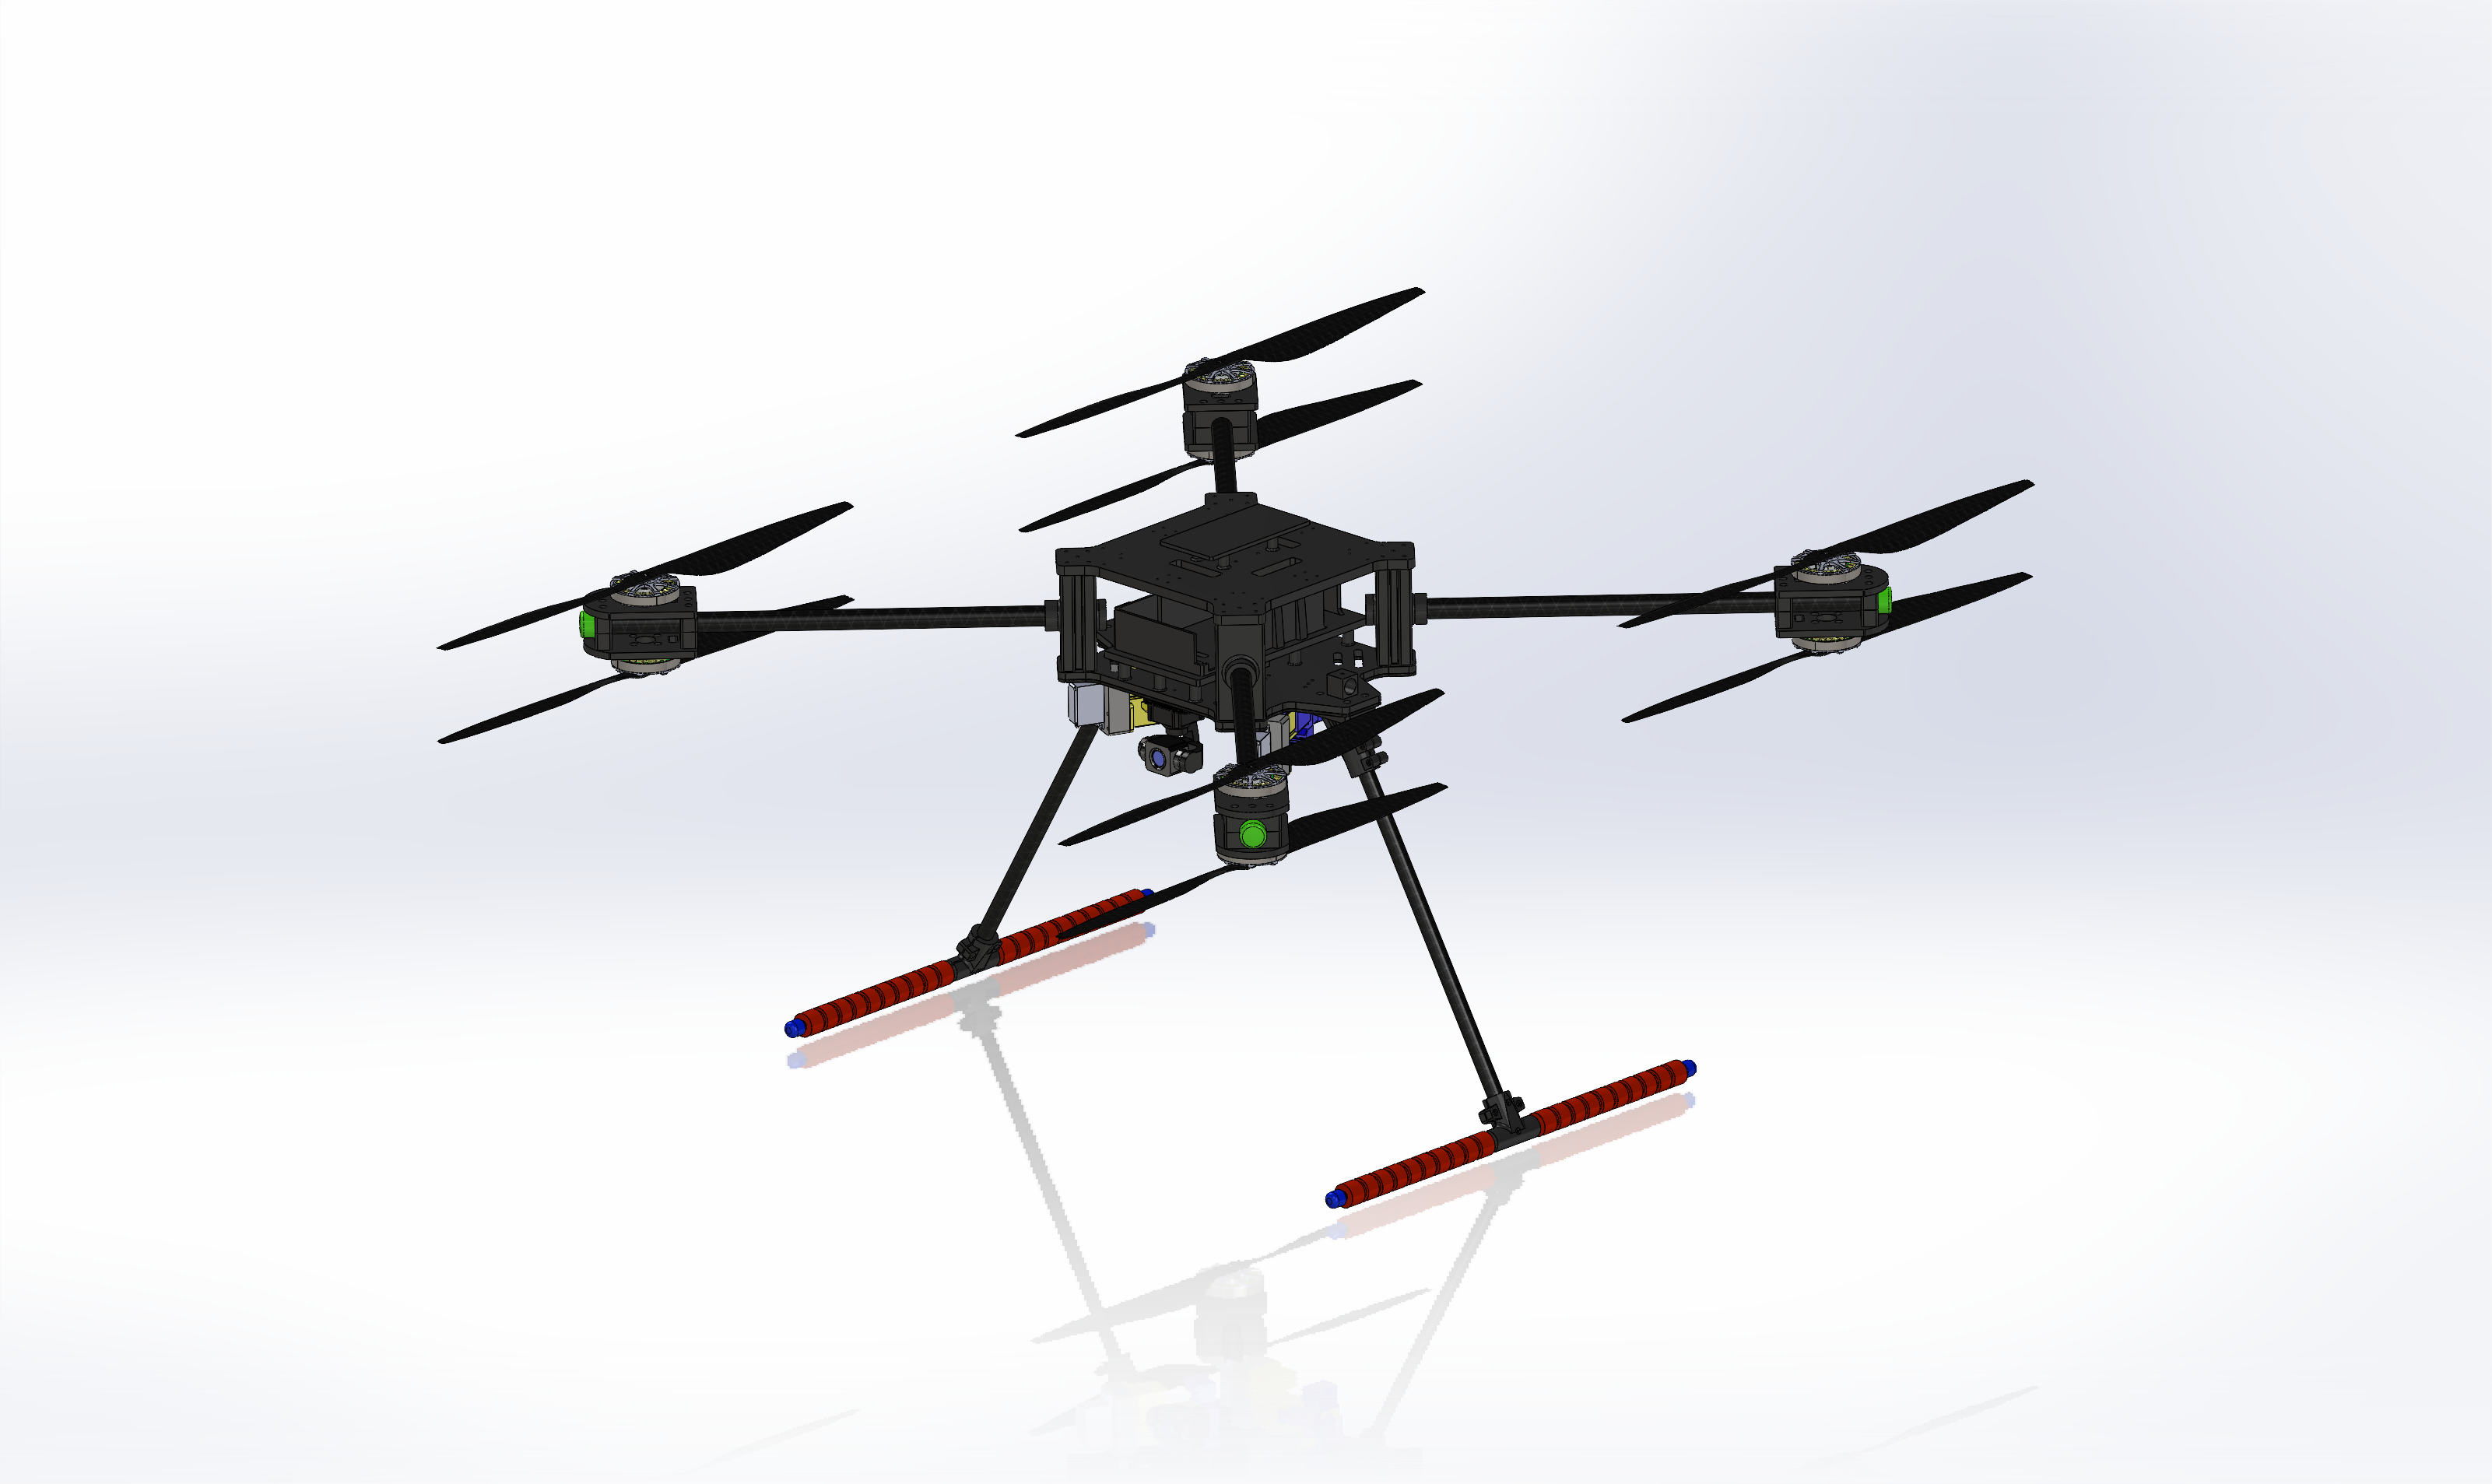
\includegraphics[width=0.85\linewidth]{figuras/montagem-drone.png}

    \vspace{0.2cm}

    \begin{flushleft}
        \footnotesize Fonte: elaboração própria.
    \end{flushleft}
\end{figure}

O modelo físico do VANT tem uma massa total de decolagem de 6,700 kg. Desse total, 6,300 kg correspondem ao corpo central da aeronave (incluindo baterias, eletrônica embarcada e o mecanismo de captura) e 0,400 kg estão divididos entre os oito conjuntos de motores e hélices (0,050 kg por rotor). Para saber como a aeronave resiste a giros em cada eixo, os momentos principais de inércia foram calculados diretamente no programa de modelagem 3D (CAD), levando em conta o volume e a densidade real de cada material aplicado no projeto, como fibra de carbono nos tubos dos braços e nas placas centrais, ligas de alumínio e cobre nos motores elétricos, células de lítio-polímero na bateria 12S e plásticos nas peças estruturais impressas em 3D. Esses cálculos definiram os valores $I_{xx} = 0{,}903322\text{ kg}\cdot\text{m}^2$, $I_{yy} = 0{,}903322\text{ kg}\cdot\text{m}^2$ e $I_{zz} = 1{,}569346\text{ kg}\cdot\text{m}^2$ em relação ao centro de massa, com produtos de inércia iguais a zero devido à simetria da estrutura.

O conjunto de motores e hélices foi calibrado no simulador com base em testes reais de bancada divulgados pela fabricante T-Motor. A configuração utiliza motores sem escovas modelo MN6007 II KV160, alimentados por uma bateria LiPo 12S com tensão nominal de 44,4 V e equipados com hélices de fibra de carbono modelo P22x6.6. A partir desses dados experimentais, foram ajustadas curvas matemáticas (por meio do método dos mínimos quadrados) para reproduzir o comportamento aerodinâmico do conjunto: a relação entre a velocidade de rotação do motor ($\omega$, em radianos por segundo) e a força de empuxo gerada ($T$, em Newtons) é descrita pela Eq.~\ref{eq:curva_empuxo_motor}, enquanto a resistência do ar ao giro da hélice, chamada de torque de arrasto ($Q$, em Newtons-metro), segue a Eq.~\ref{eq:curva_torque_motor}.

\begin{equation}
    T = c_t \cdot \omega^2 = 1{,}88928 \times 10^{-4} \cdot \omega^2
    \label{eq:curva_empuxo_motor}
\end{equation}

\begin{equation}
    Q = c_q \cdot \omega^2 = 4{,}48871 \times 10^{-6} \cdot \omega^2
    \label{eq:curva_torque_motor}
\end{equation}

Os coeficientes $c_t$ e $c_q$ obtidos no ajuste matemático reproduzem o comportamento real dos testes de bancada com uma diferença menor que 1,5\%, atingindo a velocidade máxima de rotação de 5456 RPM (571,35 rad/s) com aceleração total de 100\%, o que corresponde a um torque limite de 1,49 N$\cdot$m por eixo. No simulador, as forças aerodinâmicas que agem em cada pá das hélices foram calculadas individualmente por módulos de sustentação e arrasto (\textit{LiftDrag}), configurados com coeficiente angular de sustentação $C_{L\alpha} = 4{,}25$, coeficiente de arrasto parasita $C_{D0} = 0{,}56097$, área efetiva da pá de $0{,}0037982\text{ m}^2$ e densidade do ar padrão de $1{,}2041\text{ kg/m}^3$.

Para evitar que as imagens fiquem tremidas ou tortas, a câmera é montada em um suporte motorizado de três eixos (\textit{gimbal}), modelado com base nas características físicas do dispositivo comercial SIYI A8 mini. O conjunto pesa 0,095 kg e possui três eixos de movimento, sendo eles o eixo de guinada (\textit{yaw}), que gira entre $-160^\circ$ e $+160^\circ$, o de rolagem (\textit{roll}), que atua entre $-30^\circ$ e $+30^\circ$ e o de arfagem (\textit{pitch}), que se move entre $-135^\circ$ e $+45^\circ$. Durante a missão de captura, o \textit{gimbal} é controlado por comandos MAVLink com o travamento inercial ativado nos eixos de rolagem e arfagem. Essa configuração mantém a câmera sempre nivelada com o horizonte e apontando diretamente para baixo, perpendicular ao solo (visada nadir em $-90^\circ$), compensando as inclinações naturais que o drone faz ao se deslocar horizontalmente. Por outro lado, o eixo de guinada do \textit{gimbal} permanece travado em relação ao corpo do drone, apontando sempre para a esquerda em um ângulo fixo de $-90{,}0^\circ$ (conforme detalhado na Seção~3.5). Isso garante que qualquer giro visto na imagem corresponda exatamente à rotação real da estrutura do drone em relação ao alvo no solo.

Além disso, a câmera virtual instalada na parte inferior do \textit{gimbal} grava em resolução \textit{Full HD} de $1920 \times 1080$ pixels em cores (padrão R8G8B8), com taxa limitada a 20 quadros por segundo (fps) para acompanhar a velocidade de processamento da rede neural. O campo de visão horizontal (\textit{Horizontal FOV}) foi definido em 1,4137 radianos (cerca de $81{,}0^\circ$), o que resulta em uma distância focal teórica de $f_x = f_y = 1124{,}0$ pixels e centro óptico em $c_x = 960{,}0$ pixels e $c_y = 540{,}0$ pixels. O modelo da lente também inclui coeficientes de distorção radial ($k_1 = -0{,}05$ e $k_2 = 0{,}01$) para simular as deformações visuais típicas de lentes grande-angulares compactas.

No projeto físico do drone, a captura será feita por três garras robóticas acionadas por servomotor e instaladas na parte de baixo do \textit{frame} (\textit{underside}), projetadas para fechar sobre os pontos de encaixe da armadilha. No entanto, devido ao prazo do projeto e à alta complexidade de simular o movimento mecânico de abertura e fechamento em tempo real, essa articulação ativa não foi reproduzida no Gazebo Sim. Em vez disso, as garras foram modeladas já ligadas ao VANT, como se elas estivessem totalmente abertas, preparadas para o encaixe. Assim, assume-se e valida-se que, se o drone alcançar a posição e o alinhamento exatos dentro dessa pequena margem de erro, a garra física conseguirá fechar e prender a armadilha com firmeza.

Porém, devido ao formato do chassi e ao local onde o \textit{gimbal} é preso, a lente da câmera não fica exatamente alinhada com o centro da garra. A posição da câmera em relação ao centro do drone é definida pelo vetor $\mathbf{p}_{\text{cam}} = (0{,}00057,\, +0{,}04216,\, -0{,}04551)\text{ m}$. Enquanto a diferença lateral no eixo $X$ é menor que 0,6 mm e pode ser ignorada, o deslocamento para a frente no eixo $Y$ cria uma distância (\textit{offset}) de 42,16 mm entre a câmera e o ponto ideal de alinhamento do drone com a armadilha. Por causa disso, se o sistema tentasse alinhar a armadilha exatamente no centro da imagem da câmera ($u = c_x, v = c_y$), a garra ficaria mais de 4 centímetros atrás do ponto ideal de captura, o que faria o encaixe falhar ou causaria uma colisão com a armadilha. Essa diferença de posicionamento entre o centro da lente e o ponto ideal de alinhamento é apresentada na vista inferior da Fig.~\ref{fig:modelo_drone_offset}.

\begin{figure}[H]
    \centering
    \captionsetup{justification=centering}

    \caption{Vista inferior do VANT evidenciando o deslocamento geométrico (\textit{offset}) entre a câmera e a garra}
    \label{fig:modelo_drone_offset}

    \vspace{0.2cm}

    \includegraphics[width=0.65\linewidth]{figuras/drone-visao-de-baixo.png}

    \vspace{0.2cm}

    \begin{flushleft}
        \footnotesize Fonte: elaboração própria.
    \end{flushleft}
\end{figure}

Para compensar esse deslocamento sem exigir alterações estruturais no chassi, desenvolveu-se uma correção cinemática analítica no algoritmo de servovisão para os regimes de aproximação terminal (Fases 2 e 3). Como a tampa da armadilha possui dimensão frontal de $0{,}2550\text{ m}$, a relação entre o deslocamento da câmera e o tamanho do alvo equivale à razão da Eq.~\ref{eq:razao_offset_y}:

\begin{equation}
    \eta_y = \frac{\Delta Y_{\text{offset}}}{L_{\text{alvo}}} = \frac{0{,}04216\text{ m}}{0{,}2550\text{ m}} \approx 0{,}1653
    \label{eq:razao_offset_y}
\end{equation}

Dessa forma, o ponto de convergência visual do controlador no plano da imagem não é alinhado com o centro geométrico da caixa delimitadora predita pela rede neural, mas sim deslocado em $+16{,}53\%$ ao longo do eixo vertical de pixels proporcionalmente à altura da caixa. Essa correção analítica garante que, quando o erro de rastreamento visual converge para zero, o mecanismo físico de engate situado sob o CG do drone encontra-se rigorosamente perpendicular e alinhado às alças de captura.

O objeto-alvo não cooperativo modelado no ambiente virtual corresponde à armadilha inteligente de captura de vetores biológicos desenvolvida para o projeto VTS. A armadilha foi importada para o simulador como uma entidade dinâmica não estática, permitindo avaliar interações físicas reais de contato, atrito estático e forças de arraste mecânico durante o acoplamento da garra. A estrutura possui massa de 4,81162 kg, momentos principais de inércia $I_{xx} = 0{,}294868\text{ kg}\cdot\text{m}^2$, $I_{yy} = 0{,}150069\text{ kg}\cdot\text{m}^2$ e $I_{zz} = 0{,}258855\text{ kg}\cdot\text{m}^2$, e coeficiente de atrito superficial com o solo $\mu = 1{,}0$ sob o motor de física ODE.

A armadilha possui base circular de $0{,}127\text{ m}$ de raio e altura de $0{,}317\text{ m}$ do solo até a tampa superior. Sobre a tampa plástica, encontram-se três alças metálicas triangulares salientes destinadas ao içamento e travamento do dispositivo, conforme ilustrado na Fig.~\ref{fig:modelo_armadilha_vts}.

\begin{figure}[H]
    \centering
    \captionsetup{justification=centering}

    \caption{Modelo tridimensional renderizado da armadilha com as três alças de captura}
    \label{fig:modelo_armadilha_vts}

    \vspace{0.2cm}

    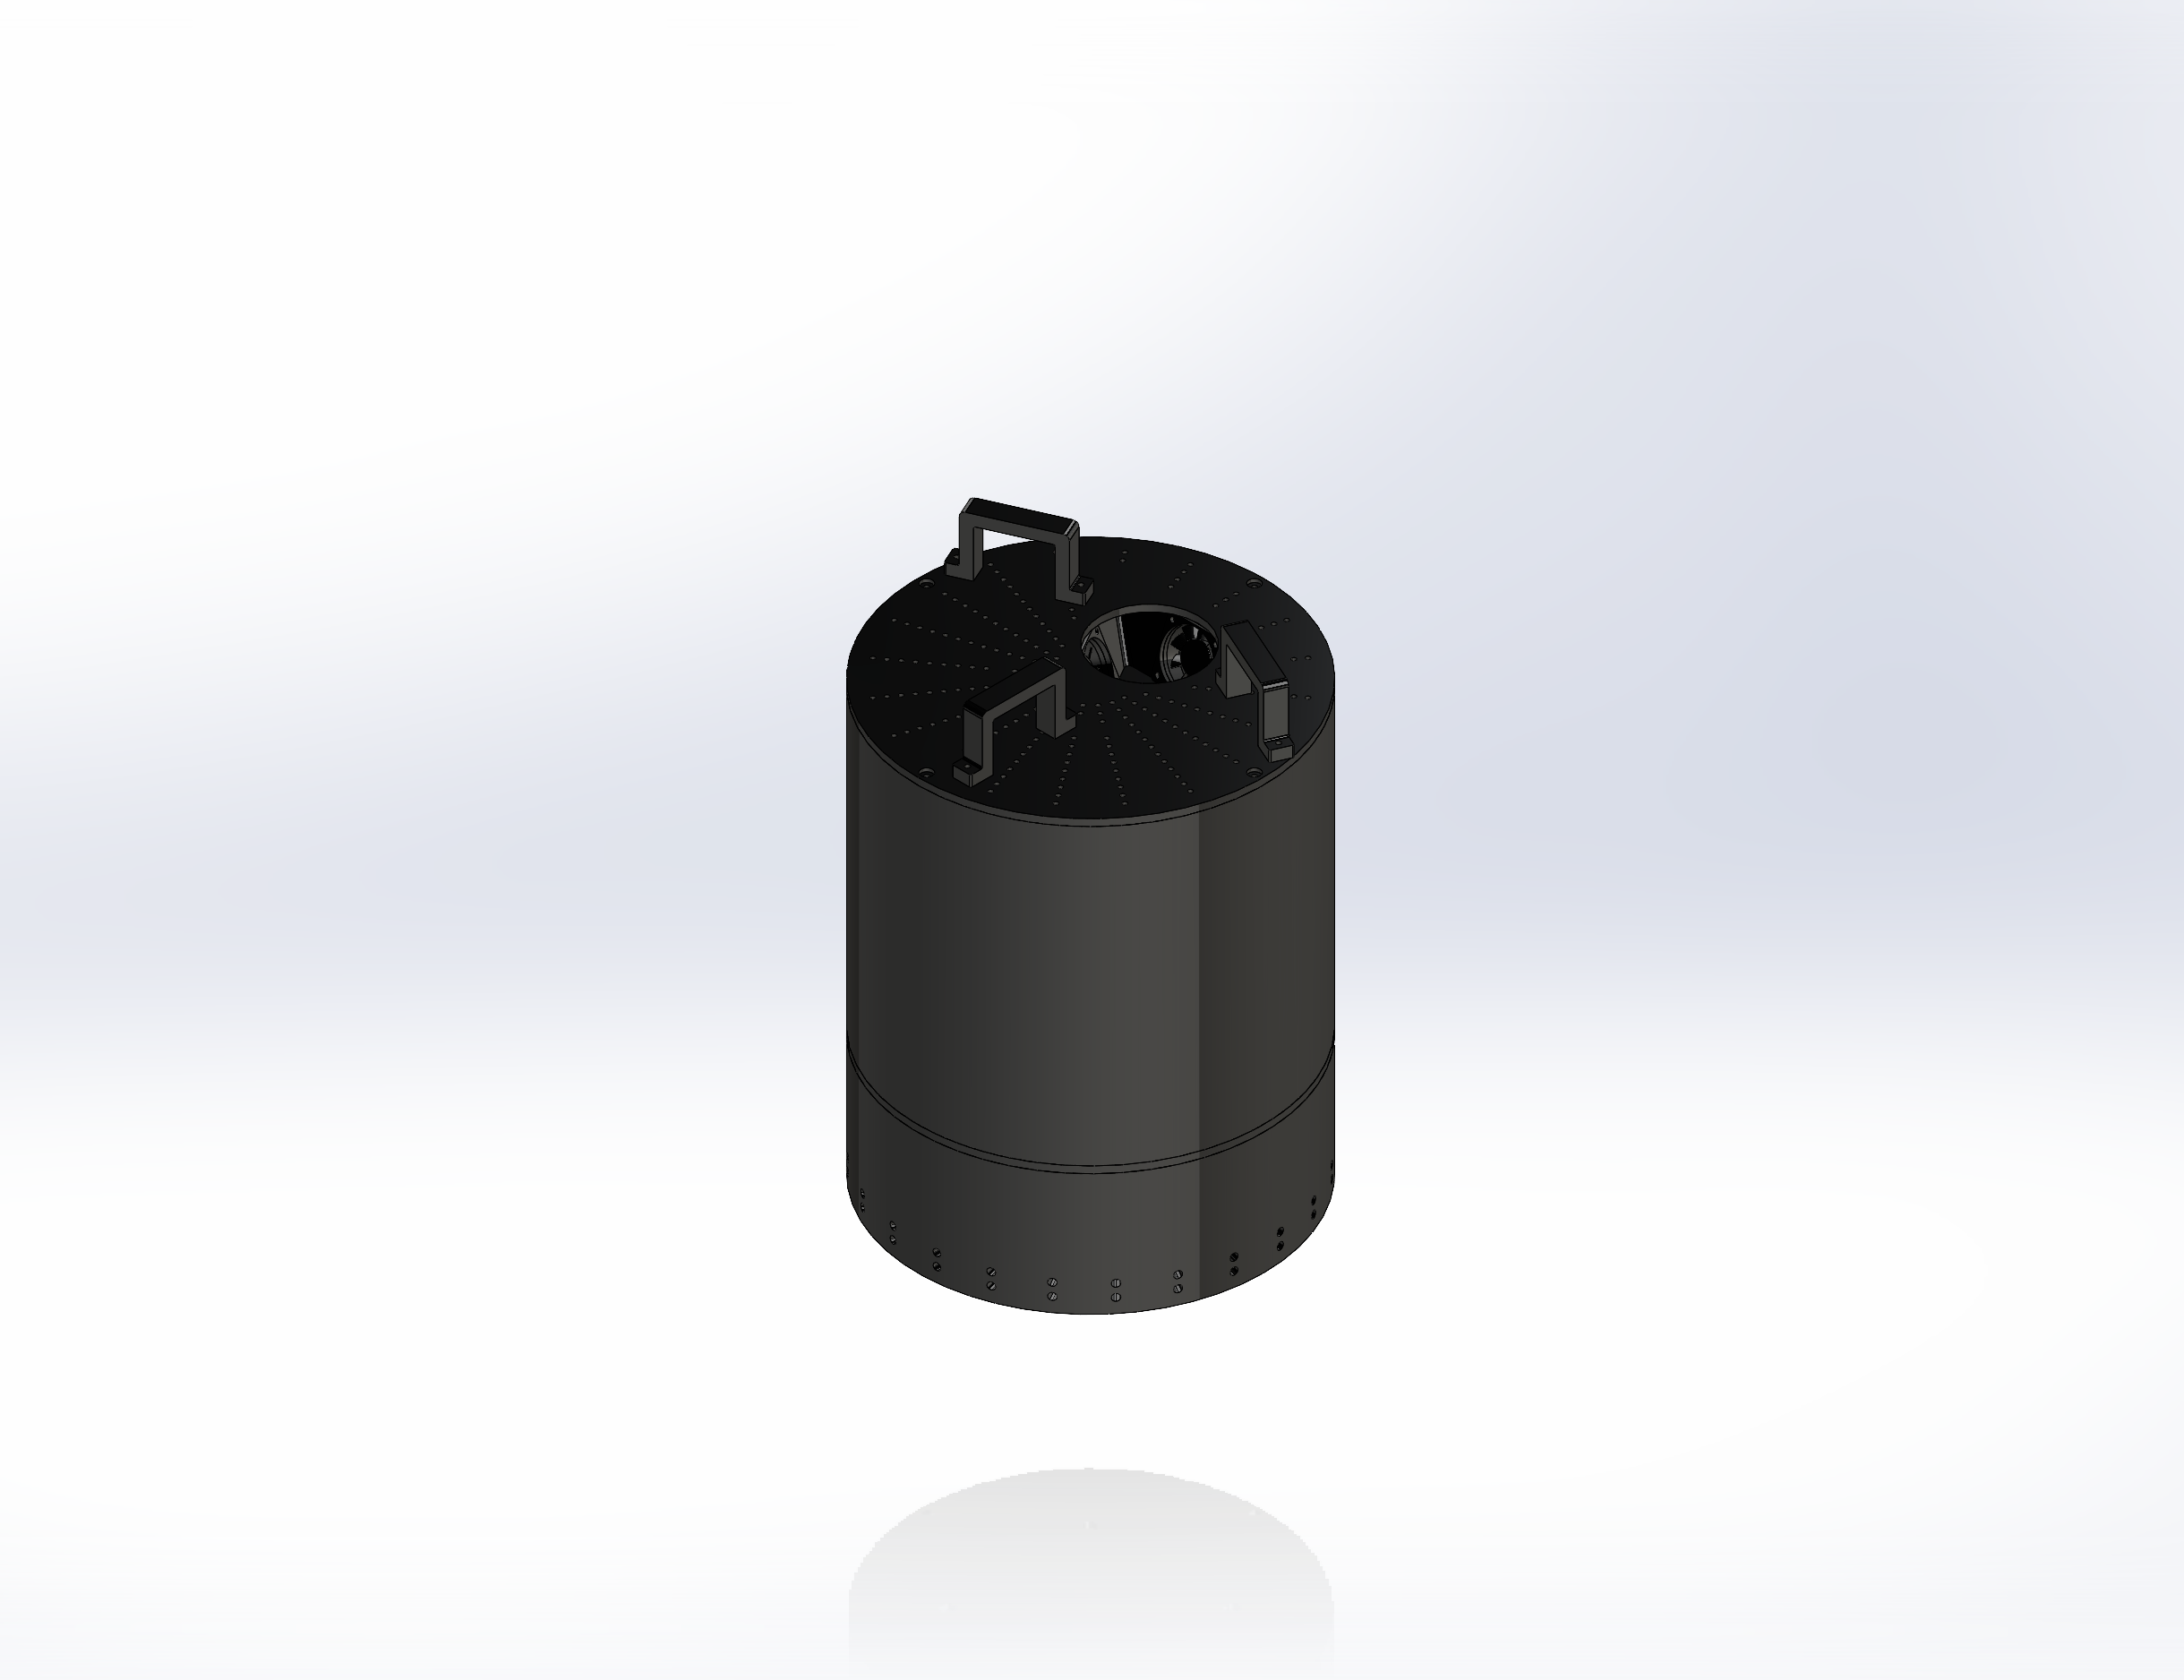
\includegraphics[width=0.85\linewidth]{figuras/montagem-armadilha.png}

    \vspace{0.2cm}

    \begin{flushleft}
        \footnotesize Fonte: elaboração própria.
    \end{flushleft}
\end{figure}

A disposição geométrica dessas três alças não é simétrica em relação aos eixos cartesianos da armadilha, apresentando uma inclinação angular de rotação de $+93{,}37^\circ$ em relação à linha de referência longitudinal da base, como evidenciado na vista superior da Fig.~\ref{fig:armadilha_visao_cima}. A presença dessa assimetria geométrica impõe um requisito mecânico determinante ao acoplamento: a abertura útil das mandíbulas da garra ventral possui tolerância angular restrita, inviabilizando abordagens em orientações arbitrárias e exigindo que a atitude de guinada da aeronave coincida estritamente com o alinhamento da armadilha para viabilizar a penetração e o travamento físico.

\begin{figure}[H]
    \centering
    \captionsetup{justification=centering}

    \caption{Vista superior da armadilha no simulador evidenciando o arranjo das alças e a inclinação de $93{,}37^\circ$}
    \label{fig:armadilha_visao_cima}

    \vspace{0.2cm}

    \includegraphics[width=0.75\linewidth]{figuras/Armadilha-visao-de-cima.png}

    \vspace{0.2cm}

    \begin{flushleft}
        \footnotesize Fonte: elaboração própria.
    \end{flushleft}
\end{figure}

A geometria desse acoplamento e a interação mecânica entre os subsistemas são mostrados na Fig.~\ref{fig:acoplamento_mecanico_lateral}. 

\begin{figure}[H]
    \centering
    \captionsetup{justification=centering}

    \caption{Representação tridimensional do acoplamento mecânico entre o VANT e a armadilha}
    \label{fig:acoplamento_mecanico_lateral}

    \vspace{0.2cm}

    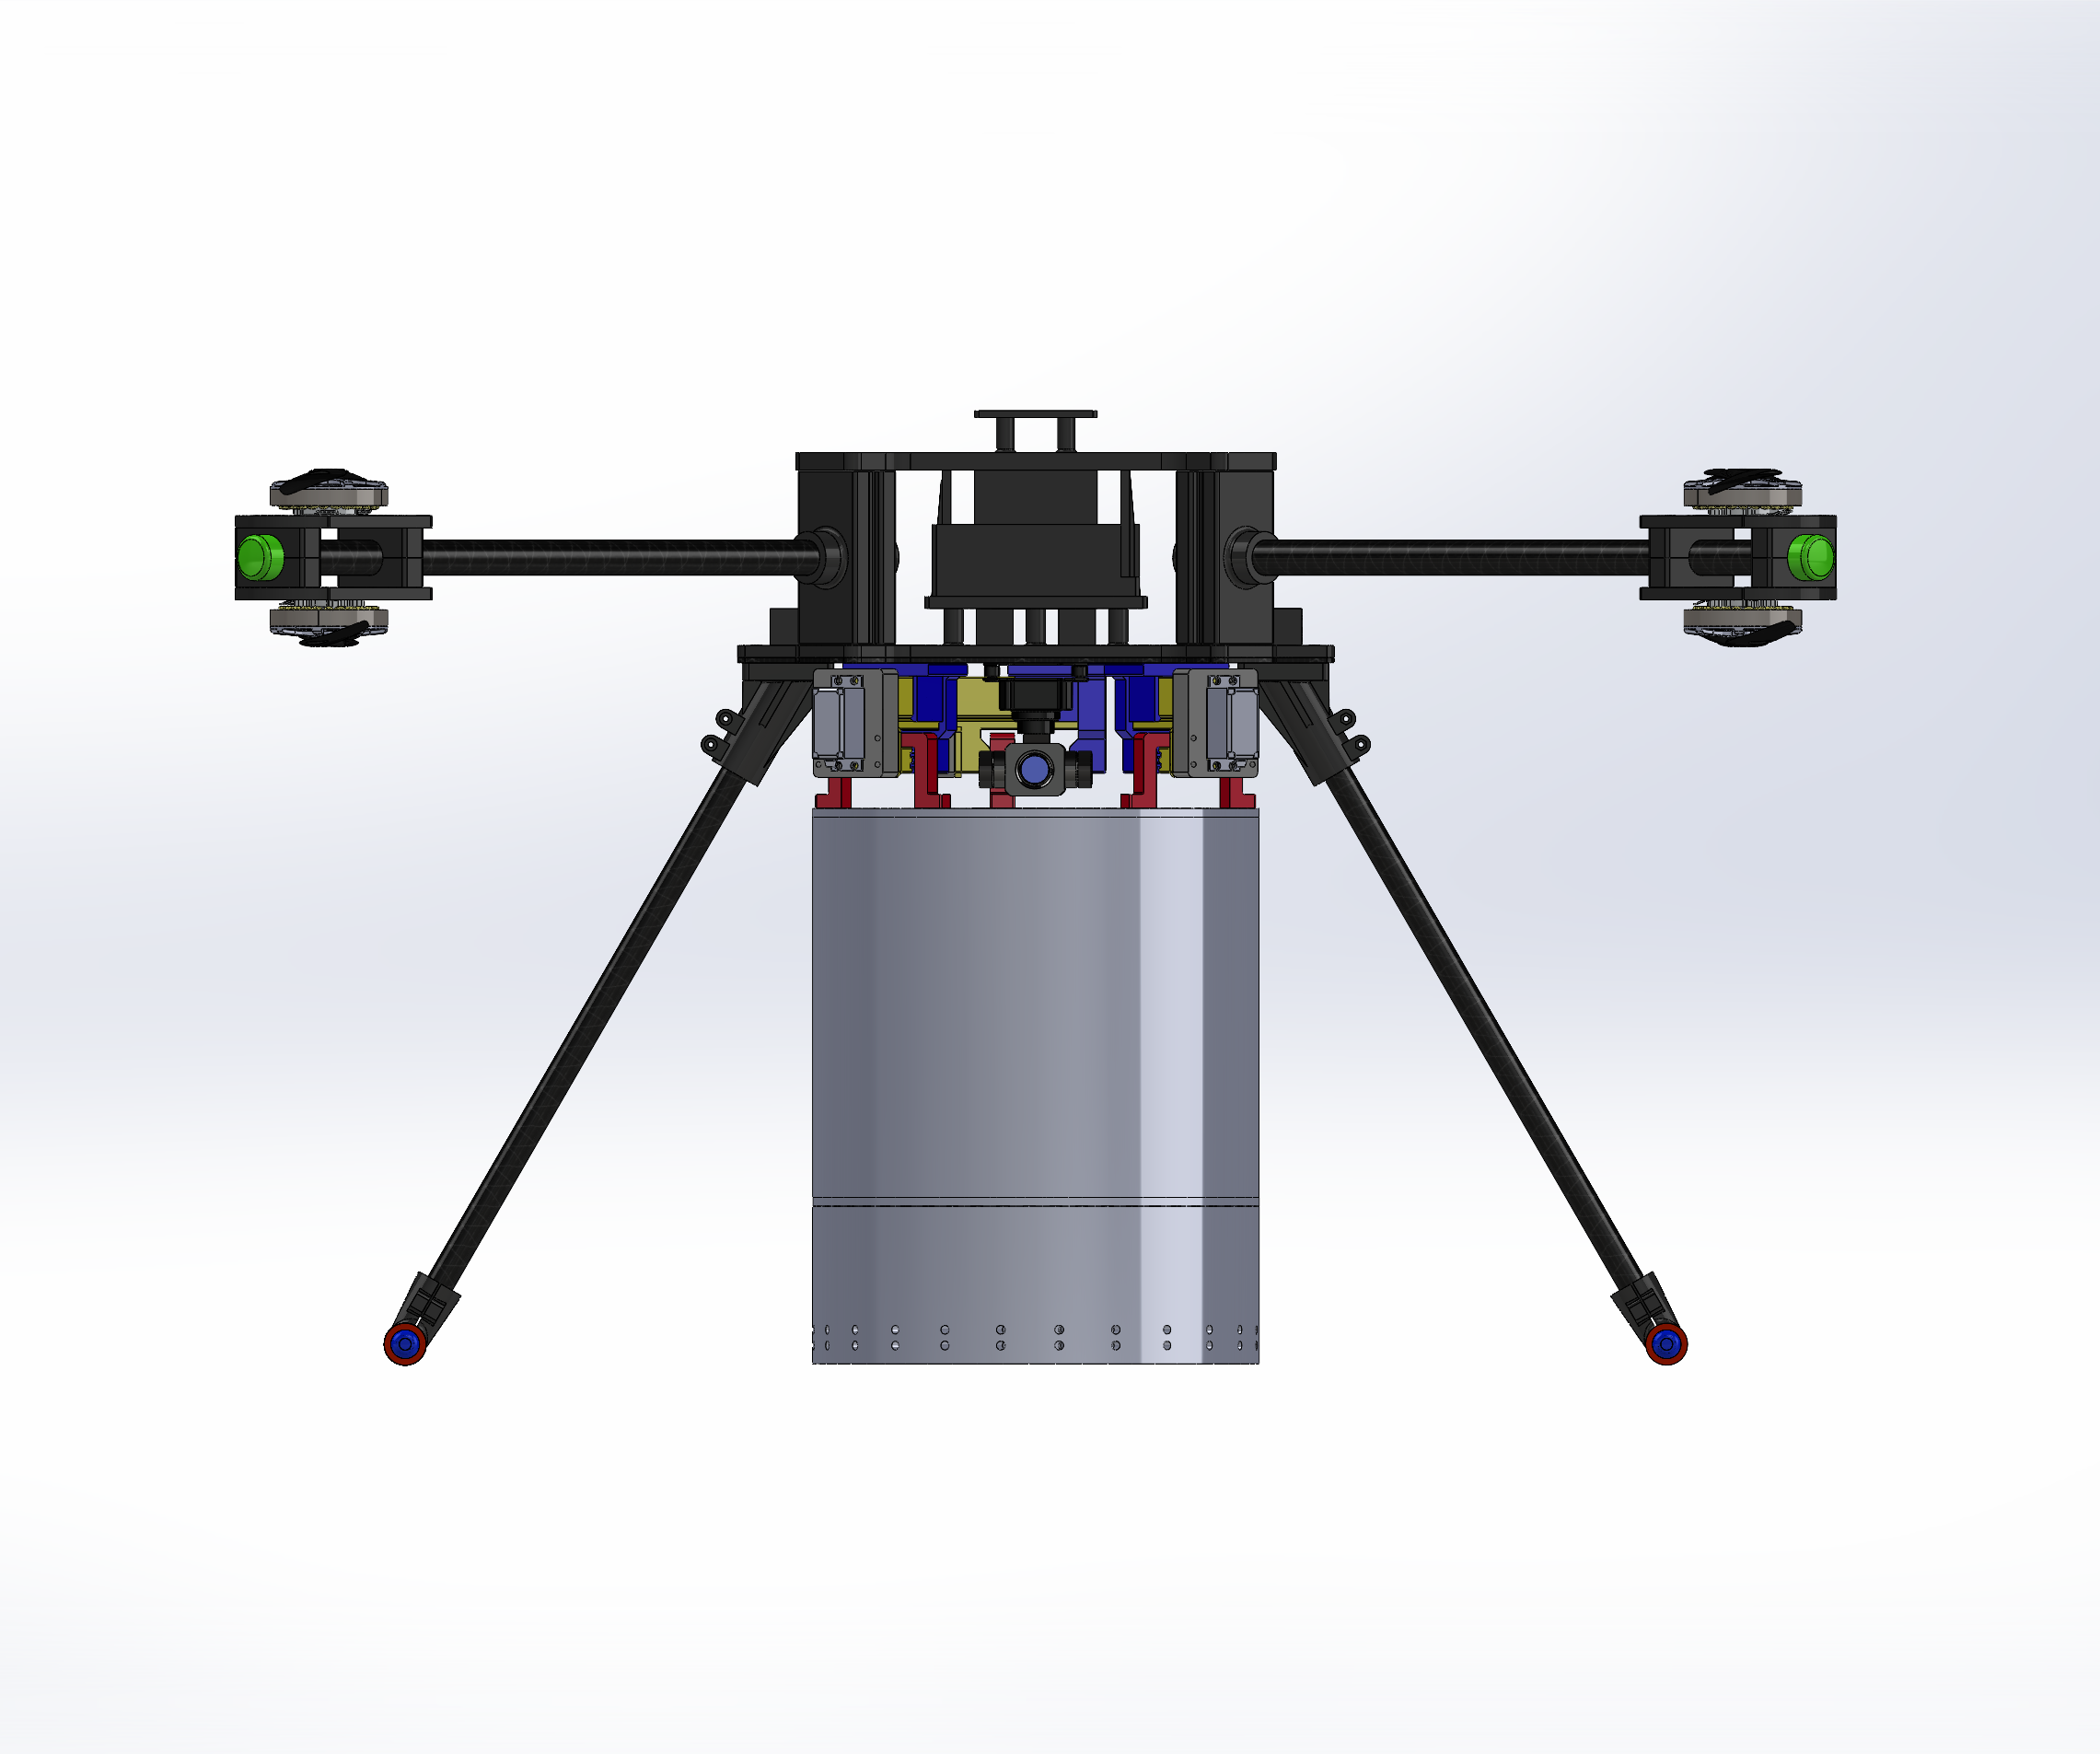
\includegraphics[width=0.85\linewidth]{figuras/montagem-drone-completa.png}

    \vspace{0.2cm}

    \begin{flushleft}
        \footnotesize Fonte: elaboração própria.
    \end{flushleft}
\end{figure}

\subsecao{\textit{Datasets} Sintéticos e Treinamento dos Detectores Visuais}

O bom funcionamento de um sistema guiado por câmera (servovisão) depende diretamente da capacidade dos modelos de inteligência artificial identificarem o alvo de forma estável ao longo do tempo, sem se confundirem com mudanças na iluminação e mantendo boa precisão em cada altura de voo. Em voos reais com drones, coletar essas imagens manualmente em campo traz grandes desafios práticos, como o risco de colidir com o chão em manobras muito baixas e a impossibilidade de controlar o clima e a posição do sol para repetir os testes nas mesmas condições. Para resolver esses problemas, optou-se por gerar bancos de imagens (\textit{datasets}) sintéticos diretamente no simulador Gazebo Sim, aproveitando a conexão integrada com o piloto automático ArduPilot para programar voos autônomos de captura de fotos. Para garantir que os contornos ficassem bem marcados e evitar os erros e falhas comuns em programas de marcação automática 3D, todas as imagens foram revisadas e rotuladas manualmente pelo próprio autor, criando caixas de detecção bem ajustadas ao formato de cada objeto.

Como a aparência e o tamanho do alvo na imagem mudam muito conforme o drone desce de 20,0 m até o encaixe físico a 0,20 m, a estratégia de visão computacional foi dividida em três conjuntos de dados independentes e complementares, voltados para três etapas visuais diferentes:

\begin{enumerate}
	\item \textbf{\textit{Dataset} da Fase 1 (Visão Geral em Funil Ótico, 20,0 m a 2,0 m):} Criado para guiar a aproximação inicial e a descida em direção ao alvo e utiliza apenas a classe \textit{armadilha}. Na coleta automática, o drone voou em trajetórias de grade retangular e ziguezague sobre o alvo em dez alturas diferentes (de 2,0 m a 20,0 m, subindo de 2,0 m em 2,0 m). Em cada altura, os movimentos laterais foram ajustados ao campo de visão da câmera voltada para baixo (nadir), fazendo a armadilha aparecer desde o centro até os cantos mais extremos da imagem. Esse conjunto reuniu 1.258 imagens, divididas em 944 para treinamento (75\%) e 314 para validação (25\%);
	
	\item \textbf{\textit{Dataset} da Fase 2 (Alinhamento Angular de Guinada / \textit{Yaw}, 2,0 m a 0,35 m):} Desenvolvido para identificar as partes assimétricas da armadilha usadas para calcular o ângulo de giro horizontal do drone e utiliza duas classes: as três alças triangulares superiores (classe \textit{alca}) e a tampa da base (classe \textit{armadilha}). As imagens foram capturadas em uma trajetória em espiral cilíndrica de raio $r = 0{,}15\text{ m}$ ao redor do centro da armadilha, subindo e descendo entre 2,0 m e 0,20 m enquanto o drone mantinha a mesma orientação fixa no espaço. O conjunto somou 546 imagens, divididas em 384 para treino (70,3\%), 107 para validação (19,6\%) e 55 para teste independente (10,1\%);
	
	\item \textbf{\textit{Dataset} da Fase 3 (Alinhamento Fino com \textit{Offset} em Ultra-Baixa Altitude, 0,35 m a 0,20 m):} Voltado especificamente para a etapa final de ajuste milimétrico das garras inferiores e utiliza apenas a classe \textit{Alinhamento}. O motivo técnico para criar esse terceiro conjunto e treinar um modelo exclusivo para a Fase 3 é explicado a seguir.
\end{enumerate}

\subsubsecao{Justificativa Física e Óptica para a Introdução do Modelo da Fase 3}

A necessidade de criar um terceiro banco de imagens (\textit{dataset}) e treinar um modelo dedicado exclusivamente à Fase 3 surge de duas limitações físicas e visuais da câmera quando o drone chega muito perto do chão:

\begin{enumerate}
	\item \textbf{Corte da Imagem nas Bordas (\textit{Edge Cropping}):} A câmera voltada para baixo (nadir) tem resolução vertical de 1080 pixels e distância focal de $f_y = 1124{,}0\text{ px}$, enquanto o corpo circular da armadilha mede $D = 0{,}2550\text{ m}$ (255 mm) de diâmetro. Pela fórmula de projeção em perspectiva $h_{\text{px}} = \frac{f_y \cdot D}{Z}$, quando o drone desce abaixo de $Z = 0{,}35\text{ m}$ de altura, a armadilha passa a ocupar $818\text{ pixels}$ na tela; ao chegar a $Z = 0{,}25\text{ m}$, ela atinge $1146\text{ pixels}$, ultrapassando o limite vertical da câmera (1080 px). Com isso, as partes de cima e de baixo da armadilha ficam cortadas fora da imagem. Quando a rede neural tenta marcar a armadilha inteira nessas condições, ela acaba criando uma caixa incompleta, o que desloca artificialmente o centro calculado $(\Delta u, \Delta v)$ em dezenas de pixels na direção da parte que ainda aparece. Esse erro de cálculo faz o sistema enviar comandos imprecisos de movimento justamente no instante mais delicado do encaixe;
	
	\item \textbf{Bloqueio Visual por Sombras do Drone:} Abaixo de 0,35 m de altura, o próprio drone \textit{OctaQuad} fica tão perto do topo da armadilha que acaba tampando a luz direta do sol. Os braços dos motores e os pés de pouso projetam sombras escuras e irregulares sobre as três alças triangulares ($30\text{ mm}$ de base). Essas sombras fazem as alças se misturarem visualmente com o plástico escuro da tampa, prejudicando a precisão do modelo da Fase 2 e impedindo o reconhecimento confiável das três alças usadas para calcular o giro do drone.
\end{enumerate}

Para resolver esses dois problemas, a Fase 3 troca o foco da visão computacional para um modelo que identifica apenas o aro circular central da tampa da armadilha (classe única \textit{Alinhamento}), que mede cerca de $72\text{ mm} \times 72\text{ mm}$. A uma altura de $Z = 0{,}20\text{ m}$, esse aro menor aparece com nitidez ocupando cerca de $400\text{ pixels}$ no centro da câmera, cabendo $100\%$ dentro da imagem mesmo quando o drone se desloca um pouco para os lados. Além disso, por ser um círculo simétrico, sua aparência não muda mesmo que o drone gire, o que permite calcular o ponto exato de encaixe com precisão milimétrica na escala de $0{,}1806\text{ mm/pixel}$.

A coleta de imagens da Fase 3 foi feita de forma automática no Gazebo Sim, com o drone subindo e descendo continuamente de forma centralizada entre 0,35 m e 0,20 m, reproduzindo fielmente as sombras reais projetadas pelo corpo do drone sobre a tampa. Ao todo, foram reunidas 400 imagens marcadas manualmente na classe \textit{Alinhamento}, divididas em 280 para treino (70,0\%), 80 para validação (20,0\%) e 40 para teste independente (10,0\%). Exemplos representativos dos três conjuntos de dados são mostrados na Fig.~\ref{fig:amostras_dataset_fases}.

\begin{figure}[H]
    \centering
    \captionsetup{justification=centering}

    \caption{Amostras representativas dos \textit{datasets} sintéticos gerados no Gazebo Sim para as Fases 1, 2 e 3}
    \label{fig:amostras_dataset_fases}

    \vspace{0.2cm}

    \includegraphics[width=0.98\linewidth]{figuras/amostras_dataset_fases.png}

    \vspace{0.2cm}

    \begin{flushleft}
        \footnotesize Fonte: elaboração própria.
    \end{flushleft}
\end{figure}

\subsubsecao{Treinamento Supervisionado e Comparativo das Arquiteturas YOLO}

O treinamento dos modelos nas três fases foi feito na plataforma Ultralytics com imagens redimensionadas para $640 \times 640$ pixels e lotes (\textit{batch size}) de 8 imagens por vez. Na Fase 1, o modelo foi treinado por 150 épocas (ciclos completos pelos dados). Na Fase 2, como era mais difícil identificar três pequenas alças muito próximas cobertas por sombras em movimento, o treinamento durou 300 épocas. Já na Fase 3 (focada no aro de alinhamento entre 0,35 m e 0,20 m), o limite foi de 200 épocas, seguindo as mesmas regras de variação de imagem (\textit{degrees} = 180, \textit{flipud} = 0,5 e \textit{fliplr} = 0,5). Em todas as fases, usou-se o otimizador AdamW com ajuste gradual da taxa de aprendizado (decaimento cossenoidal) e parada antecipada (\textit{early stopping}) caso o modelo passasse 100 épocas sem evoluir.

Para evitar que a rede neural se acostumasse apenas com os ângulos capturados durante os voos e garantir que ela reconhecesse o alvo em qualquer rotação de $360^\circ$, aplicou-se uma técnica de aumento de dados (\textit{data augmentation}) com giro aleatório completo ($\text{degrees} = 180$), rotacionando as imagens entre $-180^\circ$ e $+180^\circ$ a cada lote. O processo também incluiu mudanças de \textit{zoom} (escala), deslocamentos laterais (translações) e alterações de brilho e contraste no padrão de cores HSV, além da junção de várias fotos em mosaicos (\textit{mosaic}). Esse efeito de mosaico foi desligado nas últimas 10 épocas (\textit{close mosaic}) para que o modelo finalizasse o aprendizado com precisão sobre imagens reais e inteiras.

Para escolher as redes neurais que entregam o melhor equilíbrio entre precisão na marcação e velocidade de resposta no computador de bordo do drone, quatro versões leves e recentes da família YOLO (v8n, v10n, v11n e v26n) foram treinadas com exatamente as mesmas regras em cada uma das três fases.

Os resultados comparativos obtidos no conjunto de validação da Fase 1 são resumidos na Tab.~\ref{tab:comparativo_yolo_fase1}.

\begin{table}[H]
	\centering
	\small
	\setlength{\tabcolsep}{5pt}
	\captionsetup{justification=centering}
	\caption{Comparativo de desempenho entre arquiteturas da família YOLO na detecção macroscópica da armadilha na Fase 1 (150 épocas)}
	\label{tab:comparativo_yolo_fase1}
	\vspace{0.2cm}
	\begin{tabular}{lccccc}
		\hline
		\textbf{Arquitetura} & \textbf{Precisão ($P$)} & \textbf{\textit{Recall} ($R$)} & \textbf{$mAP@50$} & \textbf{$mAP@50\text{--}95$} & \textbf{Tempo de Treino} \\
		\hline
		YOLOv8n  & 100,00\% & 99,92\% & 99,50\% & 68,86\% & 2 h 15 min \\
		YOLOv10n & 97,62\%  & 98,23\% & 99,31\% & 70,42\% & 2 h 46 min \\
		YOLOv11n & 99,20\%  & 99,49\% & 99,48\% & 71,73\% & 2 h 32 min \\
		\textbf{YOLO26n} & \textbf{98,41\%} & \textbf{98,71\%} & \textbf{99,34\%} & \textbf{74,59\%} & \textbf{2 h 50 min} \\
		\hline
	\end{tabular}
	\vspace{0.2cm}
	\begin{flushleft}
		\footnotesize Fonte: elaboração própria.
	\end{flushleft}
\end{table}

Os dados da Tab.~\ref{tab:comparativo_yolo_fase1} mostram que, embora todas as redes tenham superado com folga a meta mínima de $mAP@50 > 90\%$, o índice mais rigoroso de precisão de contorno ($mAP@50\text{--}95$) apontou o modelo YOLO26n como a melhor escolha para a Fase 1, atingindo 74,59\% (uma vantagem de 5,73 pontos percentuais sobre o YOLOv8n). Esse encaixe mais exato da caixa de detecção evita trepidações rápidas (\textit{jitter}) no cálculo do centro da armadilha durante a descida de 20 m até 2 m.

Na Fase 2, identificar ao mesmo tempo as três alças triangulares sob sombras em movimento representou um desafio maior. A comparação entre as quatro redes treinadas para essa etapa é detalhada na Tab.~\ref{tab:comparativo_yolo_fase2}.

\begin{table}[H]
	\centering
	\small
	\setlength{\tabcolsep}{5pt}
	\captionsetup{justification=centering}
	\caption{Comparativo de desempenho entre arquiteturas da família YOLO na detecção multi-classe da Fase 2 (300 épocas)}
	\label{tab:comparativo_yolo_fase2}
	\vspace{0.2cm}
	\begin{tabular}{lccccc}
		\hline
		\textbf{Arquitetura} & \textbf{Precisão ($P$)} & \textbf{\textit{Recall} ($R$)} & \textbf{$mAP@50$} & \textbf{$mAP@50\text{--}95$} & \textbf{Tempo de Treino} \\
		\hline
		YOLOv8n  & 99,64\% & 100,00\% & 99,50\% & 82,26\% & 1 h 10 min \\
		\textbf{YOLOv10n} & \textbf{96,85\%} & \textbf{98,32\%} & \textbf{99,34\%} & \textbf{88,02\%} & \textbf{2 h 30 min} \\
		YOLOv11n & 99,20\% & 99,53\%  & 99,50\% & 87,79\% & 1 h 16 min \\
		YOLO26n  & 99,30\% & 99,21\%  & 99,47\% & 87,27\% & 2 h 01 min \\
		\hline
	\end{tabular}
	\vspace{0.2cm}
	\begin{flushleft}
		\footnotesize Fonte: elaboração própria.
	\end{flushleft}
\end{table}

Como mostra a Tab.~\ref{tab:comparativo_yolo_fase2}, o modelo YOLOv10n teve o melhor desempenho na métrica mais rigorosa ($mAP@50\text{--}95 = 88{,}02\%$). Além da boa precisão nos contornos, a escolha do YOLOv10n para a Fase 2 se deve à sua estrutura interna que dispensa o filtro tradicional chamado NMS (\textit{Dual Label Assignment}). Como as três alças ficam a poucos centímetros umas das outras, detectores comuns que dependem do NMS (como o v8n e o v11n) acabam apagando uma das alças vizinhas quando a câmera olha de lado, confundindo-a com uma marcação duplicada. Por não precisar dessa etapa de filtragem, o YOLOv10n garante o rastreamento contínuo das três alças sem falhas e com tempo de resposta previsível para o controle de giro do drone.

Por fim, o treinamento das quatro redes no conjunto de imagens da Fase 3 (alinhamento fino a 0,20 m, com a classe única \textit{Alinhamento}) foi avaliado ao longo de 200 épocas, e os resultados gerais estão na Tab.~\ref{tab:comparativo_yolo_fase3}.

\begin{table}[H]
	\centering
	\small
	\setlength{\tabcolsep}{5pt}
	\captionsetup{justification=centering}
	\caption{Comparativo de desempenho entre arquiteturas da família YOLO no treinamento da Fase 3 (alinhamento fino a 0,20 m, 200 épocas)}
	\label{tab:comparativo_yolo_fase3}
	\vspace{0.2cm}
	\begin{tabular}{lccccc}
		\hline
		\textbf{Arquitetura} & \textbf{Precisão ($P$)} & \textbf{\textit{Recall} ($R$)} & \textbf{$mAP@50$} & \textbf{$mAP@50\text{--}95$} & \textbf{Menor \textit{Box Loss}} \\
		\hline
		YOLOv8n  & 99,93\% & 100,00\% & 99,50\% & 95,75\% & 0,2939 \\
		\textbf{YOLOv10n} & \textbf{99,93\%} & \textbf{100,00\%} & \textbf{99,50\%} & \textbf{99,50\%} & \textbf{0,1759} \\
		YOLOv11n & 99,93\% & 100,00\% & 99,50\% & 99,50\% & 0,1996 \\
		YOLO26n  & 99,93\% & 100,00\% & 99,50\% & 99,50\% & 0,1347 \\
		\hline
	\end{tabular}
	\vspace{0.2cm}
	\begin{flushleft}
		\footnotesize Fonte: elaboração própria.
	\end{flushleft}
\end{table}

A análise da Tab.~\ref{tab:comparativo_yolo_fase3} confirma que simplificar a tarefa para detectar apenas o aro circular central permitiu um aprendizado quase perfeito. Os modelos YOLOv10n, YOLOv11n e YOLO26n atingiram o teto máximo de $99{,}50\%$ tanto em $mAP@50$ quanto em $mAP@50\text{--}95$, com erros mínimos no ajuste das caixas ($\text{Box Loss} < 0{,}26$), enquanto o YOLOv8n parou em $95{,}75\%$.

Para rodar no sistema embarcado durante a Fase 3, o modelo YOLOv10n foi novamente escolhido como o detector oficial. Ele combina a precisão máxima de $99{,}50\%$ com um tempo de processamento de apenas $35{,}0\text{ ms}$ por imagem ($28{,}6\text{ fps}$) e não utiliza o filtro NMS. A 0,20 m de altura, onde qualquer atraso ou oscilação na detecção tiraria as garras da pequena margem de encaixe ($\le 8\text{ mm}$), a rapidez e a estabilidade do YOLOv10n garantem a precisão necessária para o acoplamento antes da descida final sem câmera (\textit{Blind Drop}).

A evolução e a estabilidade do aprendizado dos modelos selecionados ao longo das épocas de treinamento podem ser observadas na Fig.~\ref{fig:curvas_treinamento_yolo}, que apresenta o comportamento das perdas de regressão e classificação, bem como a progressão dos índices de precisão média.


\begin{figure}[H]
    \centering
    \captionsetup{justification=centering}

    \caption{Curvas de aprendizado dos modelos selecionados nas três fases ao longo das épocas de treinamento}
    \label{fig:curvas_treinamento_yolo}

    \vspace{0.2cm}

    \includegraphics[width=0.92\linewidth,height=0.75\textheight,keepaspectratio]{figuras/curvas_treinamento_yolo.png}

    \vspace{0.2cm}

    \begin{flushleft}
        \footnotesize Fonte: elaboração própria.
    \end{flushleft}
\end{figure}

\subsecao{Implementação da Filtragem Estocástica de Estados (EKF)}

Usar apenas uma câmera para guiar o drone traz desafios práticos ligados à divisão da imagem em pixels, às mudanças de luz e contraste na cena e às vibrações mecânicas da própria estrutura da aeronave. Embora as caixas de detecção geradas pelos modelos YOLO identifiquem o alvo com alta precisão média, a posição exata do ponto central sofre pequenas oscilações rápidas (\textit{jitter}) de um quadro para o outro. Se essas coordenadas brutas fossem enviadas diretamente para o controle de voo, os motores receberiam comandos irregulares e fariam o drone tremer. Além disso, a câmera informa apenas a posição do alvo, e tentar calcular a velocidade a partir da diferença simples entre uma imagem e outra ampliaria muito esses pequenos ruídos visuais.

Para resolver esses problemas sem pesar no computador de bordo, foi criado um módulo de filtragem baseado no Filtro de Kalman Estendido (EKF), cujos fundamentos foram explicados na Seção~2.3. Na prática, esse filtro funciona como um sistema de tratamento de sinais responsável por três tarefas principais:
\begin{enumerate}
	\item Suavizar as coordenadas do alvo, reduzindo as pequenas oscilações rápidas (\textit{jitter}) geradas pela rede neural;
	\item Calcular de forma contínua a velocidade de aproximação e a velocidade de giro do drone, permitindo que os controladores PD trabalhem com respostas amortecidas e sem ruídos;
	\item Manter a estimativa da trajetória do drone por cálculo inercial (\textit{dead reckoning}) caso a câmera perca o alvo de vista por instantes rápidos, como quando a sombra do próprio drone cobre a armadilha em baixa altitude.
\end{enumerate}

Na estrutura de software desenvolvida no ROS 2, a filtragem foi dividida em dois módulos complementares ligados ao controle de voo e sincronizados na taxa de 20 Hz ($\Delta t = 0{,}05\text{ s}$):

O primeiro módulo, chamado \textit{FiltroAlvoEKF}, cuida do rastreamento horizontal da armadilha. Ele recebe as posições medidas no plano horizontal ($x$ e $y$) e estima as velocidades de aproximação ($v_x$ e $v_y$). Na prática, o filtro foi ajustado por meio de testes para equilibrar dois fatores essenciais: o quanto o sistema confia nas medições da câmera e a inércia natural do movimento do drone. Assim, o algoritmo ignora os pequenos tremores momentâneos da caixa de detecção e mantém o voo suave. Quando o drone desce abaixo de 0,35 m de altura e troca para o detector de alinhamento final (onde cada pixel passa a valer frações de milímetro), o filtro muda automaticamente para um modo de resposta mais rápido. Isso permite corrigir pequenos desvios finais com precisão milimétrica, sem deixar de filtrar as vibrações da estrutura.

O segundo módulo, chamado \textit{FiltroAnguloEKF}, é dedicado exclusivamente ao alinhamento de giro horizontal (\textit{Yaw}) na Fase 2, onde é obrigatório atingir um erro menor que $1{,}0^\circ$ para que a garra inferior consiga se encaixar. Esse filtro acompanha o ângulo da armadilha ($\theta$) e a velocidade de rotação ($\omega$). Para evitar falhas matemáticas quando o ângulo cruza a transição entre $+180^\circ$ e $-180^\circ$ (o que causaria um salto brusco nos números e faria o drone dar uma volta completa desnecessária e violenta), o algoritmo calcula automaticamente a correção pelo caminho angular mais curto. Esse cuidado garante que o ajuste de direção aconteça sempre pelo percurso mais rápido, suave e estável.

Outro recurso importante criado no filtro é o tratamento automático para quando o alvo fica temporariamente encoberto. Na parte final da descida (abaixo de 1,50 m de altura), o drone fica bem entre o sol e a armadilha, projetando sombras escuras sobre a tampa que podem esconder por alguns instantes as alças ou o corpo do objeto. Sempre que o modelo YOLO falha em detectar o alvo em um quadro, o EKF pausa a leitura da câmera e passa a prever a posição apenas com base no movimento anterior. Nesse modo, o sistema continua informando a posição estimada aos controladores usando a inércia e a velocidade que o drone já tinha, permitindo que a descida continue suave e nivelada.

Para garantir a segurança da operação, foi configurado um limite de tempo de 4,0 segundos seguidos sem sinal visual (o que equivale a 80 ciclos seguidos a 20 Hz). Se a armadilha voltar a aparecer dentro desse prazo, o filtro volta a usar os dados da câmera de forma gradual, corrigindo qualquer pequena diferença acumulada sem dar trancos no drone. Porém, se a perda de imagem passar de 4,0 segundos, o sistema ativa uma rotina de segurança (\textit{reset}), zera os cálculos internos do filtro e faz o drone interromper a descida, ficando parado no ar (voo pairado) em segurança até receber um novo comando.

\subsecao{Reconstrução Geométrica 3D e Controle Cinemático}

Para converter a posição do alvo vista em pixels na tela em distâncias reais no espaço 3D (abordagem PBVS), o sistema utiliza o modelo matemático inverso de câmera \textit{Pinhole}. A partir do ponto central suavizado pelo filtro EKF $(\tilde{u}, \tilde{v})$, as distâncias horizontais em metros $(x_m, y_m)$ até o alvo no solo são calculadas pela Eq.~\ref{eq:pinhole_inverso}
\begin{equation}
	x_m = \frac{(\tilde{u} - c_x) \cdot Z}{f_x}, \quad y_m = \frac{(\tilde{v} - c_y) \cdot Z}{f_y}
	\label{eq:pinhole_inverso}
\end{equation}
onde os dados internos da lente são lidos automaticamente pelo tópico \texttt{/camera/\allowbreak camera\_info} do ROS~2 na resolução \textit{Full HD} ($1920 \times 1080$ px), usando centro óptico $(c_x, c_y) = (960{,}0;\, 540{,}0)\text{ px}$ e distâncias focais $f_x = f_y = 1124{,}0\text{ px}$.

O valor da distância vertical $Z$ usada nessa conta muda conforme a altitude do drone. Na Fase 1 (entre 20,0 m e 2,0 m), a altura da própria armadilha é muito pequena comparada à altura de voo e não exige uma precisão perfeita na transformação, então usa-se diretamente a altitude do drone em relação ao chão, $Z = Z_{\text{alt}}$. Já nas Fases 2 e 3 (abaixo de 2,0 m), por ter que ajustar o ângulo a partir das alças que se encontram na parte de cima da armadilha e por já estar bem mais perto do chão, o sistema passa a calcular a distância exata entre a lente da câmera e a tampa superior da armadilha por meio da Eq.~\ref{eq:profundidade_relativa_fase2}
\begin{equation}
	Z_{\text{rel}} = \max\left(0{,}005;\; (Z_{\text{alt}} + h_{\text{camera}}) - h_{\text{alvo}}\right)
	\label{eq:profundidade_relativa_fase2}
\end{equation}
em que $h_{\text{camera}} = 0{,}320\text{ m}$ é a altura da lente em relação aos pés de pouso do drone e $h_{\text{alvo}} = 0{,}317\text{ m}$ é a altura da armadilha até a tampa, mantendo um valor mínimo de $0{,}005\text{ m}$ para evitar falhas de divisão por zero. É necessário obter os valores de $h_{\text{camera}}$ pelo fato de a altitude ser marcada como a distância do chão até o trem de pouso. Além disso, como o \textit{gimbal} aponta diretamente para baixo (visada nadir) e fica travado a $-90{,}0^\circ$ em relação à frente do drone (alinhado ao lado esquerdo), os deslocamentos medidos na imagem correspondem diretamente aos eixos de movimento da aeronave (\texttt{MAV\_FRAME\_BODY\_NED}): o desvio horizontal $X_{\text{img}}$ ($x_m$) controla a velocidade para frente e para trás ($v_x$), o desvio vertical $Y_{\text{img}}$ ($y_m$) controla a velocidade para os lados ($v_y$), e a altura governa a velocidade de descida ($v_z$).

Durante a descida rápida da Fase 1, uma regra de segurança dividida em duas áreas na tela impede que o drone perca a armadilha de vista. Se o centro do alvo se afastar do meio da imagem ($W/2 = 960\text{ px}$, $H/2 = 540\text{ px}$) e ultrapassar a margem limite de $60\%$, o drone interrompe a descida ($v_z = 0{,}0\text{ m/s}$) para focar apenas em se centralizar sobre o alvo, voltando a descer somente quando a armadilha retorna para a área segura interna de $40\%$. Enquanto a descida acontece, a velocidade base $v_{z,\text{base}}$ diminui gradualmente a partir do valor máximo de $v_{z,\text{nom}} = 1{,}50\text{ m/s}$ conforme o alvo se aproxima da borda de $60\%$ (respeitando um mínimo de 20\%) e também é suavizada por uma rampa de desaceleração entre 6,0 m e 2,0 m de altura, definida pela Eq.~\ref{eq:fator_frenagem}:
\begin{equation}
	f_{\text{frenagem}} = \max\left(0{,}10;\; \min\left(1{,}0;\; \frac{Z_{\text{alt}} - 2{,}0}{6{,}0 - 2{,}0}\right)\right), \quad v_z = v_{z,\text{base}} \cdot f_{\text{frenagem}}
	\label{eq:fator_frenagem}
\end{equation}

Na Fase 2 (a 1,50 m de altura), o ajuste de giro do drone usa como referência as três alças triangulares da tampa. Depois de eliminar marcações repetidas sobre o mesmo ponto ($\text{IoU} > 0{,}05$, $\text{IoA} > 0{,}10$ ou distância menor que $0{,}06\text{ m}$) para ter certeza de que está detectando 3 alças diferentes, o sistema define os três pontos principais $(P_0, P_1, P_2)$, identifica a ponta principal do triângulo formado por eles (\textit{Apex}, definida pelos dois lados adjacentes mais simétricos) e calcula a direção apontada desde o meio da base até essa ponta. Esse ângulo passa pelo filtro \textit{FiltroAnguloEKF} e é comparado pelo caminho mais curto em $[-\pi, \pi]$ com o ângulo de referência calibrado de $\theta_{\text{alvo}} = +93{,}37^\circ$ ($1{,}6296\text{ rad}$, Fig.~\ref{fig:armadilha_visao_cima}), exigindo que o erro angular fique dentro de $|e_\psi| \le 1{,}0^\circ$ por pelo menos $0{,}30\text{ s}$ seguidos. Como mecanismo de segurança para o drone não parar em uma posição que ele não consiga detectar as 3 alças corretamente, se a detecção de alguma dessas alças falhar por mais de $3{,}0\text{ s}$, o sistema aplica um giro lento de $\omega = 0{,}25\text{ rad/s}$ para mudar o ângulo de visão e tentar voltar a enxergar as peças.

Terminado o alinhamento de giro a 1,50 m, ainda na etapa final da Fase 2, o sistema inicia a correção por software da diferença de posição (\textit{offset}) entre a câmera e a garra ($Y_{\text{offset}} = -0{,}04216\text{ m}$ e $X_{\text{offset}} = 0{,}0000\text{ m}$), sem exigir modificações físicas no drone. Durante essa descida entre 1,50 m e 0,35 m de altura, usa-se o fator de proporção $\eta_y \approx 0{,}1653$ da Eq.~\ref{eq:razao_offset_y} multiplicado pela altura da caixa de detecção da armadilha $h_{\text{box}}$ (suavizada por média móvel exponencial EMA com $\alpha = 0{,}50$) para deslocar o ponto de mira na imagem conforme a Eq.~\ref{eq:alvo_virtual_offset}. Ao cruzar a altura de 0,35 m, inicia-se efetivamente a Fase 3 (de 0,35 m até 0,20 m). Nessa etapa, como as sombras do drone e os cortes nas bordas da imagem atrapalham a visão da tampa inteira, o detector troca para a classe \textit{Alinhamento} (focada apenas no aro central de $72\text{ mm} \times 72\text{ mm}$ na escala de $5{,}5\text{ px/mm}$, com EMA $\alpha = 0{,}55$), aplicando os ajustes milimétricos calibrados ($\eta_{x,\text{alin}} = +0{,}0034$ e $\eta_{y,\text{alin}} = +0{,}0121$) definidos pela Eq.~\ref{eq:alvo_virtual_alinhamento}:
\begin{equation}
	u_{\text{alvo}} = u_{\text{gaiola}}, \quad v_{\text{alvo}} = v_{\text{gaiola}} - (h_{\text{box}} \cdot \eta_y)
	\label{eq:alvo_virtual_offset}
\end{equation}
\begin{equation}
	u_{\text{alvo}} = u_{\text{alin}} + (w_{\text{box}} \cdot \eta_{x,\text{alin}}), \quad v_{\text{alvo}} = v_{\text{alin}} - (h_{\text{box}} \cdot \eta_{y,\text{alin}})
	\label{eq:alvo_virtual_alinhamento}
\end{equation}

O controle automático de movimento usa controladores proporcional-derivativos (PD) independentes operando a 20 Hz ($\Delta t = 0{,}05\text{ s}$) para calcular as velocidades horizontais ($v_x, v_y$, a partir dos erros de distância $e_x, e_y$ em metros) e a velocidade de giro ($\omega$, a partir do erro angular $e_\psi$ em radianos), seguindo a fórmula com limite máximo da Eq.~\ref{eq:controle_pd}
\begin{equation}
	u(t) = \text{sat}\left(K_p \cdot e(t) + K_d \cdot \frac{e(t) - e(t - \Delta t)}{\Delta t},\; u_{\max}\right)
	\label{eq:controle_pd}
\end{equation}
cujos parâmetros e limites variam conforme cada etapa do voo, como detalhado na Tab.~\ref{tab:ganhos_controle_pd}. Durante a descida guiada pelo aro central (de $0{,}35\text{ m}$ até $0{,}20\text{ m}$), o drone pausa a descida ($v_z = 0{,}0\text{ m/s}$) se a câmera perder o alvo de vista ou se o erro lateral passar de 40 mm. Depois de concluir o alinhamento fino a 0,20 m (com velocidade horizontal limitada a no máximo $35\text{ mm/s}$), o sistema trava a posição horizontal no referencial fixo do terreno (\texttt{MAV\_FRAME\_LOCAL\_NED}) e executa a descida final sem câmera (\textit{Blind Drop}) a $v_z = 0{,}80\text{ m/s}$ até tocar o solo e concluir a captura.

\begin{table}[H]
	\centering
	\small
	\setlength{\tabcolsep}{5pt}
	\captionsetup{justification=centering}
	\caption{Ganhos e limites de saturação do controle cinemático PD por fase operacional}
	\label{tab:ganhos_controle_pd}
	\vspace{0.2cm}
	\begin{tabular}{lcccc}
		\hline
		\textbf{Regime Operacional} & \textbf{Saída} & \textbf{$K_p$} & \textbf{$K_d$} & \textbf{Saturação ($u_{\max}$)} \\
		\hline
		Fase 1: Funil (20,0 m -- 2,0 m)                & $v_x, v_y$ & 0,40 & 0,01 & 1,50 m/s \\
		Fase 2: Alinhamento a 1,50 m                   & $v_x, v_y$ & 0,15 & 0,05 & 0,25 m/s \\
		Fase 2: Controle de Guinada a 1,50 m           & $\omega$   & 0,40 & 0,10 & 0,40 rad/s \\
		Fase 2: Descida c/ \textit{offset} (1,50 m -- 0,35 m)   & $v_x, v_y$ & 0,15 & 0,05 & 0,35 m/s \\
		Fase 3: Descida no aro (0,35 m -- 0,20 m)      & $v_x, v_y$ & 0,15 & 0,05 & 0,25 m/s \\
		Fase 3: Ancoragem fina a 0,20 m                & $v_x, v_y$ & 0,22 & 0,08 & 0,035 m/s \\
		\hline
	\end{tabular}
	\vspace{0.2cm}
	\begin{flushleft}
		\footnotesize Fonte: elaboração própria.
	\end{flushleft}
\end{table}

O funcionamento conjunto dessas etapas de visão computacional, filtragem e controle durante o voo pode ser acompanhado em tempo real na tela de monitoramento em OpenCV mostrada na Fig.~\ref{fig:visao_opencv_tres_fases}, que exibe a imagem inteira da câmera à esquerda e uma ampliação do centro à direita para cada uma das três fases. Em (a) (Fase 1, a 5,8 m de altura), aparecem a margem interna de segurança (40\%), o limite externo de fuga (60\%), a caixa de detecção da armadilha e o ponto central suavizado pelo filtro EKF já alinhado com a mira. Em (b) (Fase 2, a 1,40 m), o sistema reconhece e conecta em triângulo as três alças superiores acompanhadas pelo EKF (\textit{P0}, \textit{P1} e \textit{P2}) para calcular o giro do drone. Já em (c) (Fase 3, a 0,26 m), nota-se a troca para o modelo da classe \textit{Alinhamento} focado no aro circular interno, mostrando a distância proposital entre o ponto exato de encaixe da garra (\textit{ALVO (ALINHAMENTO)}) e o centro da lente da câmera (\textit{MIRA (Centro Camera)}) devido à correção do \textit{offset}.

\begin{figure}[H]
	\centering
	\captionsetup{justification=centering}
	
	\caption{Interface de monitoramento em OpenCV nas três fases de aproximação}
	\label{fig:visao_opencv_tres_fases}
	
	\vspace{0.2cm}
	
	\includegraphics[width=0.95\linewidth,height=0.76\textheight,keepaspectratio]{figuras/visao_opencv_tres_fases.png}
	
	\vspace{0.2cm}
	
	\begin{flushleft}
		\footnotesize Fonte: elaboração própria.
	\end{flushleft}
\end{figure}

\subsecao{Supervisão da Missão e Máquina de Estados}

Para organizar a passagem entre as diferentes etapas do voo e garantir que a missão aconteça de forma autônoma, foi criada uma estrutura baseada em Máquina de Estados Finitos (FSM, do inglês \textit{Finite State Machine}). Essa máquina de estados funciona como o gerenciador principal do sistema, ficando responsável por iniciar os módulos (nós) no ROS 2, trocar os modelos de rede neural na memória da placa de vídeo (GPU), enviar comandos ao piloto automático ArduPilot pelo protocolo MAVLink e lidar com imprevistos caso a câmera perca o alvo de vista por alguns instantes.

O funcionamento lógico da missão é mostrado na Fig.~\ref{fig:maquina_estados_missao}, que reúne os oito estados de operação, as regras de distância e tempo para mudar de uma etapa para outra, os ciclos de controle e as rotinas de segurança utilizadas.

\begin{figure}[H]
	\centering
	\captionsetup{justification=centering}
	
	\caption{Diagrama da máquina de estados e fluxo operacional da missão autônoma}
	\label{fig:maquina_estados_missao}
	
	\vspace{0.2cm}
	
	\includegraphics[width=0.98\linewidth]{figuras/maquina_estados_missao.png}
	
	\vspace{0.2cm}
	
	\begin{flushleft}
		\footnotesize Fonte: elaboração própria.
	\end{flushleft}
\end{figure}

A missão foi dividida em oito estados de operação (Estados 0 a 7):

\textbf{Estado 0 (Configuração de Pré-Voo e Parâmetros Iniciais):} A missão começa estabelecendo a comunicação de telemetria UDP pelo endereço local \texttt{udp:\allowbreak 127.\allowbreak 0.\allowbreak 0.\allowbreak 1:\allowbreak 14550}, verificando o sinal contínuo de conexão (\textit{heartbeat}) do MAVLink com um prazo máximo de 15 segundos. O sistema aguarda os sensores do drone ligarem e se estabilizarem até que o ArduPilot confirme a variável \texttt{is\_armable}, indicando que os giroscópios, acelerômetros e o GPS estão calibrados e prontos.

Em seguida, o gerenciador envia ajustes iniciais ao piloto automático pelo comando \texttt{PARAM\_SET}. Configura-se \texttt{WP\_YAW\_BEHAVIOR = 0} (para manter a frente do drone travada na mesma direção durante os deslocamentos) e define-se \texttt{LAND\_SPD\_MS = 0,8} m/s como a velocidade de descida no pouso. Ao mesmo tempo, o \textit{gimbal} recebe o comando MAVLink \texttt{MAV\_CMD\_\allowbreak DO\_\allowbreak GIMBAL\_\allowbreak MANAGER\_\allowbreak PITCHYAW}, apontando a câmera diretamente para baixo ($\theta_{\text{pitch}} = -90{,}0^\circ$) e girada a $\psi_{\text{gimbal}} = -90{,}0^\circ$ em relação à frente do drone (alinhada com o lado esquerdo). As travas \texttt{ROLL\_LOCK} e \texttt{PITCH\_LOCK} são ativadas para compensar as inclinações do corpo do drone, aplicando-se uma pequena pausa de 0,25 segundos para estabilização.

\textbf{Estado 1 (Decolagem e Subida Inicial):} O sistema muda o modo de voo para guiado (\texttt{GUIDED}) e liga os motores (\texttt{vehicle.armed = True}). Logo depois, inicia a decolagem vertical automática (\texttt{simple\_takeoff}). Nos testes de Monte Carlo, a altura inicial de voo $Z_{\text{inicial}}$ foi sorteada entre 16,0 m e 20,0 m ($Z_{\text{inicial}} \sim \mathcal{U}(16{,}0; 20{,}0)\text{ m}$), simulando as variações de altura com que o drone chegaria em uma operação real em campo. O drone sobe até cumprir a condição da Eq.~\ref{eq:criterio_decolagem}:
\begin{equation}
	Z_{\text{alt}} \ge 0{,}95 \cdot Z_{\text{inicial}}
	\label{eq:criterio_decolagem}
\end{equation}
na qual $Z_{\text{alt}}$ indica a altura medida pelo barômetro em relação ao solo. Ao atingir 95\% da altura definida, a aeronave para de subir, estabiliza no ar e encerra a etapa de decolagem.

\textbf{Estado 2 (Navegação e Perturbação de GPS):} Em missões reais em campo, as coordenadas iniciais da armadilha vêm de receptores de GPS comuns, que sempre apresentam pequenas margens de erro na localização. Para reproduzir essa situação, foi adicionado um desvio aleatório ao redor da posição real da armadilha ($X_0 = 50{,}0\text{ m}, Y_0 = 0{,}0\text{ m}$), sorteando uma distância radial $r_{\text{erro}} \sim \mathcal{U}(1{,}0; 4{,}5)\text{ m}$ e uma direção $\theta_{\text{erro}} \sim \mathcal{U}(0, 2\pi)\text{ rad}$. O limite máximo de 4,5 m garante que, mesmo no pior cenário de imprecisão do GPS, a armadilha ainda apareça dentro da imagem da câmera na altura inicial de voo.

As coordenadas no padrão ENU (\textit{East-North-Up}) do simulador Gazebo são convertidas para o sistema local NED (\textit{North-East-Down}) usado pelo ArduPilot, gerando as posições $N_{\text{alvo}} = Y_0 + r_{\text{erro}} \sin\theta_{\text{erro}}$ e $E_{\text{alvo}} = X_0 + r_{\text{erro}} \cos\theta_{\text{erro}}$. O voo horizontal até esse ponto é monitorado até que a distância restante cumpra a Eq.~\ref{eq:distancia_residual_gps}:
\begin{equation}
	d_{\text{GPS}} = \sqrt{(N_{\text{drone}} - N_{\text{alvo}})^2 + (E_{\text{drone}} - E_{\text{alvo}})^2} \le 1{,}20\text{ m}
	\label{eq:distancia_residual_gps}
\end{equation}
estabelecendo como critério de chegada estar a menos de 1,20 m do alvo estimado, dentro de um prazo máximo de segurança de 25,0 segundos.

Assim que chega a essa região, a máquina de estados comanda um giro aleatório na horizontal ($\psi_{\text{inicial}} \sim \mathcal{U}(0{,}0^\circ; 360{,}0^\circ)$) pelo comando \texttt{MAV\_CMD\_CONDITION\_YAW}, justamente para testar se o sistema consegue se alinhar partindo de qualquer direção de chegada. Depois disso, o drone aguarda 5,0 segundos parado no ar (voo pairado) para eliminar qualquer balanço residual antes de começar a etapa guiada pela câmera.

\textbf{Estado 3 (Servovisão Macro - Fase 1):} Com o drone estabilizado, entra em ação o módulo \texttt{RastreadorYOLO} no ROS 2, que passa a enviar comandos de velocidade 20 vezes por segundo (20 Hz) baseados na orientação do próprio drone (\texttt{MAV\_FRAME\_BODY\_NED}). A rede neural YOLO26n analisa as imagens da câmera voltada para baixo para encontrar a armadilha e enviar sua posição ao filtro EKF.

Esse estado conta com duas rotinas complementares:
\begin{enumerate}
	\item Descida controlada por margem de segurança na tela (histerese visual): regula a velocidade de descida $v_z$ conforme explicado na Seção~3.5, pausando a descida caso a armadilha chegue muito perto das bordas da imagem e voltando a descer assim que o drone se centralizar novamente sobre o alvo;
	\item Busca ativa em 3D caso o alvo suma da tela: se a rede neural parar de detectar a armadilha, o drone fica parado no ar por 2,5 segundos para ter certeza de que não foi apenas uma falha rápida causada por reflexos de luz. Se o alvo continuar desaparecido, inicia-se uma manobra de busca de 18,0 segundos (voando a $0{,}50\text{ m/s}$ na horizontal e $0{,}40\text{ m/s}$ na vertical). O formato dessa trajetória é mostrado na Fig.~\ref{fig:varredura_busca_3d}: o drone faz movimentos de ida e volta para os lados no eixo Y (de 0 a 6,0 s), para frente e para trás no eixo X (de 6,0 a 12,0 s) e sobe e desce no eixo Z (de 12,0 a 18,0 s), variando a altura entre 3,0 m e 22,0 m para aumentar a área vista pela câmera até localizar a armadilha novamente.
\end{enumerate}

O critério para encerrar a Fase 1 depende da altura do drone, conforme a Eq.~\ref{eq:condicao_transicao_fase1}:
\begin{equation}
	Z_{\text{alt}} \le 2{,}00\text{ m}
	\label{eq:condicao_transicao_fase1}
\end{equation}
Assim que chega a 2,00 m de altura, o drone zera todas as velocidades ($v_x = v_y = v_z = 0{,}0\text{ m/s}$), salva os registros de permanência do alvo no campo de visão e encerra esse módulo de visão com um comando \texttt{SystemExit}.

\begin{figure}[H]
	\centering
	\captionsetup{justification=centering}
	
	\caption{Trajetória tridimensional de busca adotada em contingência de perda do alvo}
	\label{fig:varredura_busca_3d}
	
	\vspace{0.2cm}
	
	\includegraphics[width=0.98\linewidth]{figuras/varredura_busca_3d.png}
	
	\vspace{0.2cm}
	
	\begin{flushleft}
		\footnotesize Fonte: elaboração própria.
	\end{flushleft}
\end{figure}

\textbf{Estado 4 (Transição e Comutação de Nós no ROS 2):} Para passar da aproximação geral para o alinhamento de precisão, o gerenciador da missão encerra o módulo \texttt{RastreadorYOLO}, fecha as janelas de visualização do OpenCV e remove o modelo YOLO26n da memória da GPU. Logo em seguida, inicia o módulo \texttt{RastreadorFinoYOLO}, carregando na memória os modelos YOLOv10n da Fase 2 (para identificar as alças e a armadilha) e da Fase 3 (focado no aro central para o ajuste fino abaixo de 0,35 m). Dividir o sistema em duas etapas evita sobrecarregar a placa de vídeo e garante que o processamento continue rodando a 20 Hz. A partir desse ponto, o ROS 2 passa a executar o novo módulo.

\textbf{Estado 5 (Alinhamento Angular de Guinada - Fase 2):} Ao assumir o controle, o módulo \texttt{RastreadorFinoYOLO} ativa o modelo YOLOv10n capaz de identificar várias classes ao mesmo tempo. O drone desce de 2,00 m até 1,50 m mantendo a armadilha centralizada na tela e para no ar para girar na horizontal até atingir o ângulo calibrado de $+93{,}37^\circ$, deixando as alças perfeitamente alinhadas com a abertura da garra. O sistema só avança para a próxima fase quando o drone cumpre a condição de alinhamento angular da Eq.~\ref{eq:criterio_trava_yaw}:
\begin{equation}
	|e_{\psi}| \le 1{,}00^\circ \quad \text{durante} \quad \Delta t_{\text{yaw}} \ge 0{,}30\text{ s}
	\label{eq:criterio_trava_yaw}
\end{equation}
o que equivale a 6 leituras seguidas a 20 Hz dentro da margem de erro de um grau. Caso a sombra do próprio drone esconda alguma alça por mais de 3,0 segundos, comanda-se um giro lento de $\omega = 0{,}25\text{ rad/s}$ para mudar a posição da sombra e recuperar a visão das peças.

\textbf{Estado 6 (Alinhamento Fino e Ancoragem Terminal - Fase 3):} Terminado o alinhamento de giro a 1,50 m e descendo para a altitude de 0,35 m, o sistema inicia a Fase 3, executando a aproximação final e corrigindo a distância (\textit{offset}) entre a câmera e a garra em três etapas:
\begin{enumerate}
	\item Descida com \textit{offset} (de 1,50 m até 0,35 m): o ponto de mira passa a ser o Ponto de Captura Virtual (Eq.~\ref{eq:alvo_virtual_offset}), deslocado $+42{,}16\text{ mm}$ atrás da câmera no eixo longitudinal. O drone desce mantendo a garra alinhada até cruzar a altura $Z_{\text{alt}} \le 0{,}35\text{ m}$;
	\item Descida guiada pelo aro central (de 0,35 m até 0,20 m): o sistema troca para o modelo da classe \textit{Alinhamento} e ajusta os parâmetros do filtro EKF para respostas mais rápidas. O drone desce guiado pelo centro do aro interno (Eq.~\ref{eq:alvo_virtual_alinhamento}) reduzindo a velocidade aos poucos. Por segurança, a descida é pausada ($v_z = 0{,}0\text{ m/s}$) caso o aro suma da câmera ou o erro lateral passe de 40 mm;
	\item Ancoragem a 0,20 m e descida cega: ao chegar a 0,20 m de altura, o drone estabiliza parado no ar ($v_z = 0{,}0\text{ m/s}$). A descida final sem câmera só é liberada quando a aeronave cumpre a condição de precisão da Eq.~\ref{eq:criterio_hover_etapa4b}:
	\begin{equation}
		\|e_{xy}\| = \sqrt{e_x^2 + e_y^2} \le 0{,}005\text{ m} \; (5\text{ mm}), \quad \Delta t \ge 2{,}50\text{ s}, \quad Z_{\text{alt}} \le 0{,}20\text{ m}
		\label{eq:criterio_hover_etapa4b}
	\end{equation}
	o que exige 50 quadros seguidos a 20 Hz dentro de uma margem de erro menor que 5 mm. Cumprida essa exigência, o sistema trava a posição horizontal no referencial fixo do solo (\texttt{LOCAL\_NED}) e comanda uma descida vertical firme a $v_z = 0{,}80\text{ m/s}$ (\textit{blind drop}) até atingir o limite de contato da Eq.~\ref{eq:criterio_blind_drop}:
	\begin{equation}
		Z_{\text{alt}} \le 0{,}025\text{ m} \quad \text{ou} \quad Z_{\text{rel}} \le 0{,}025\text{ m} \quad (25\text{ mm})
		\label{eq:criterio_blind_drop}
	\end{equation}
	ou perceber que o drone parou de descer ao encostar no topo da armadilha ($Z_{\text{alt}} \le 0{,}06\text{ m}$ com variação menor que 4 mm durante 0,60 s), encerrando então o módulo de visão com o comando \texttt{raise SystemExit}.
\end{enumerate}

\textbf{Estado 7 (Pouso, Desarme e Armazenamento dos Dados):} Encerrada a fase guiada por câmera, o controle passa para a rotina de finalização. O piloto automático muda para o modo de pouso (\texttt{LAND}, descendo na velocidade ajustada em \texttt{LAND\_SPD\_MS = 0,8} m/s) até confirmar que os motores foram desligados (\texttt{vehicle.armed == False}).

Depois do pouso, o gerenciador consulta as coordenadas exatas do simulador Gazebo Sim (\textit{ground truth}) para calcular o erro real de posicionamento após o toque no solo ($e_x, e_y$ e $\text{RMSE}$), além de salvar os resultados registrados antes da descida final sem câmera (\textit{Blind Drop}). Todos os dados de cada teste são gravados no arquivo \texttt{relatorio\_testes\_monte\_carlo.csv} e nas pastas de telemetria.

A evolução ao longo do tempo e as mudanças de altura durante os oito estados de uma missão completa sem falhas são mostradas no gráfico de perfil de voo da Fig.~\ref{fig:perfil_voo_missao}. A curva destaca a descida contínua do drone e mostra claramente as pausas no ar para o alinhamento de giro a 1,50 m e para o ajuste fino a 0,20 m, etapas que acontecem logo antes da descida vertical final e do pouso seguro no chão.

\begin{figure}[H]
	\centering
	\captionsetup{justification=centering}
	
	\caption{Perfil de altitude e transição dos estados operacionais ao longo da missão}
	\label{fig:perfil_voo_missao}
	
	\vspace{0.2cm}
	
	\includegraphics[width=0.85\linewidth]{figuras/perfil_voo_missao.png}
	
	\vspace{0.2cm}
	
	\begin{flushleft}
		\footnotesize Fonte: elaboração própria.
	\end{flushleft}
\end{figure}

\subsecao{Protocolo Experimental e Definição dos Ensaios de Validação}

Para comprovar na prática o cumprimento dos sete objetivos específicos apresentados na Introdução, foi montada uma bateria automatizada com cinco testes complementares. Essa rotina combina avaliações numéricas feitas fora de voo (\textit{offline}) sobre os bancos de imagens e filtros reais com simulações completas em malha fechada no simulador físico Gazebo Sim integrado ao piloto automático ArduPilot SITL.

\begin{enumerate}
	\item \textbf{Teste 1: Avaliação Comparativa e Desempenho em Tempo Real dos Detectores YOLO (Objetivos 1 e 2):} As quatro arquiteturas leves (YOLOv8n, YOLOv10n, YOLOv11n e YOLO26n) passam por testes separados após o treinamento em cada etapa: Fases 1 e 2 (\texttt{teste\_1\_\allowbreak benchmark\_\allowbreak yolo.py}) e Fase 3 a 0,20 m de altura (\texttt{teste\_benchmark\_\allowbreak etapa3\_\allowbreak alinhamento.py}). Para comprovar o Objetivo 1, são medidos os índices de Precisão ($P$), \textit{Recall} ($R$), $mAP@50$ (com meta mínima acima de $90\%$) e $mAP@50\text{--}95$; para validar o Objetivo 2, mede-se o tempo médio de resposta para cada imagem (latência em milissegundos) e a velocidade de processamento quadro a quadro (\textit{batch} = 1, com meta mínima acima de $20\text{ fps}$). Na Fase 3 a 0,20 m, também são avaliadas medidas detalhadas de precisão espacial nos conjuntos de validação e teste, como a sobreposição média (\textit{IoU} contínuo), o erro de distância do centro do alvo em pixels e em milímetros na escala de 0,20 m, o percentil P95, o erro máximo e o desvio médio de direção.
	
	\item \textbf{Teste 2: Validação Estocástica e em Malha Fechada do Filtro EKF (Objetivo 3):} Realizado em duas etapas complementares para testar de forma rigorosa a suavização dos ruídos da câmera e de ângulo, além da capacidade do filtro manter a trajetória prevista por até 4,0 segundos sem visão, conforme previsto no Objetivo 3:
	\begin{itemize}
		\item \textit{Bateria de Monte Carlo offline} (\texttt{teste\_2\_\allowbreak validacao\_\allowbreak ekf.py}): executa $N = 50$ simulações independentes com duração de 17,5 s a 20 Hz (350 ciclos) diretamente sobre os módulos reais \textit{FiltroAlvoEKF} e \textit{FiltroAnguloEKF}, aplicando deriva horizontal aleatória, giro contínuo que cruza propositalmente o limite angular de $\pm 180^\circ$ ($S^1$), ruído gaussiano ($\sigma_{xy} = 35\text{ mm}$, $\sigma_\psi = 3{,}5^\circ$) e falhas pontuais abruptas (\textit{outliers} periódicos de $\pm 120\text{ mm}$ / $\pm 100\text{ mm}$ / $\pm 10^\circ$). O teste é dividido em quatro momentos: visão ativa ($0{,}0\text{ a } 5{,}0\text{ s}$), bloqueio total da câmera por $4{,}00\text{ s}$ ($5{,}0\text{ a } 9{,}0\text{ s}$, 80 ciclos), retomada da visão ($9{,}0\text{ a } 11{,}5\text{ s}$) e bloqueio prolongado acima do limite de segurança ($11{,}5\text{ a } 16{,}0\text{ s}$ com retorno visual em $16{,}0\text{ s}$). Verifica-se a redução das oscilações (\textit{jitter}) em pelo menos $40\%$, o funcionamento contínuo em 100\% dos 80 ciclos sem câmera, desvio acumulado $\le 250\text{ mm}$, erro na retomada $\le 60\text{ mm}$, reinicialização automática (\textit{reset}) após $4{,}0\text{ s}$ e estabilização pós-\textit{reset} $\le 80\text{ mm}$;
		\item \textit{Ensaio de oclusão em malha fechada}: voo completo no Gazebo Sim (executando \texttt{main.py} com \texttt{-{}-teste-\allowbreak oclusao} e o \textit{script} \texttt{teste\_2\_\allowbreak simulador\_\allowbreak analise.py}) em um cenário isolado do conjunto de Monte Carlo do Teste 5. O ensaio grava ao mesmo tempo os dados brutos do YOLO sem filtro e os dados suavizados pelo EKF a 20 Hz (para medir a redução das vibrações de alta frequência por segunda diferença na posição $XY$ e no giro) e provoca um apagão proposital da câmera durante a descida com deslocamento (\textit{offset}) da Fase 3 (por cerca de $3{,}8\text{ s}$, logo abaixo do limite de 4,0 s), avaliando a estabilidade do voo e as posições reais do drone no simulador Gazebo antes, logo após o corte de imagem, na volta da visão e ao término do pouso.
	\end{itemize}
	
	\item \textbf{Teste 3: Retenção no Campo de Visão e Histerese Visual (Objetivo 4):} Durante a descida em funil da Fase 1 em todos os voos simulados, o sistema acompanha continuamente a posição do alvo convertida pelo modelo \textit{Pinhole} em relação às bordas da tela ($0\%$ no centro da câmera até $100\%$ nas extremidades da imagem), registrando a taxa de permanência completa do alvo no campo de visão (FOV, com meta rigorosa de $100\%$ prevista no Objetivo 4), a maior aproximação registrada em relação ao limite de fuga de $60\%$ e o número de pausas verticais acionadas pela regra de segurança visual (histerese).
	
	\item \textbf{Teste 4: Controle em Cascata e Alinhamento Autônomo de Guinada (Objetivo 5):} Avaliado durante o ajuste de giro da Fase 2 (a 1,50 m de altura) e na conclusão do pouso, verificando o funcionamento estável do controle em diferentes velocidades de resposta (400 Hz no ArduPilot SITL e 20 Hz no módulo do ROS 2) e o cumprimento da meta rigorosa de ângulo do Objetivo 5 de $|e_\psi| < 1{,}0^\circ$ ($\le 1{,}0^\circ$ no critério de parada do controle), registrando a média, o desvio padrão e o maior erro observado em toda a bateria de testes.
	
	\item \textbf{Teste 5: Bateria Estocástica de Monte Carlo da Missão Completa e Acoplamento (Objetivos 6 e 7):} Comprova de ponta a ponta os resultados finais exigidos nos Objetivos 6 e 7 por meio de uma série mínima de $N \ge 20$ missões autônomas completas no simulador Gazebo integrado ao ArduPilot SITL (totalizando 60 voos realizados com reinicialização completa do ambiente físico e do piloto automático entre cada ensaio). Em cada voo são sorteados aleatoriamente a altura inicial de cruzeiro ($16{,}0\text{ a } 20{,}0\text{ m}$), o erro radial do GPS ($1{,}0\text{ a } 4{,}5\text{ m}$ em qualquer direção $[0, 2\pi)$) e o ângulo inicial de orientação do drone ($0{,}0^\circ\text{ a } 360{,}0^\circ$). Ao final da descida vertical sem câmera e do pouso completo em modo \texttt{LAND}, a precisão do encaixe é medida diretamente pelas coordenadas reais do mundo simulado (\textit{ground truth} do Gazebo entre o chassi do drone e a armadilha), verificando se o erro médio radial final fica abaixo de $\text{RMSE} < 8{,}0\text{ mm}$ sobre o ponto de captura (Objetivo 6), junto com a permanência de $100\%$ do alvo no campo de visão e erro angular $|e_\psi| \le 1{,}0^\circ$, tendo como meta geral uma taxa de sucesso superior a $60\%$ nas missões completas (Objetivo 7, consolidada pelo \textit{script} \texttt{teste\_3\_4\_5\_\allowbreak analise\_\allowbreak monte\_\allowbreak carlo.py}).
\end{enumerate}

O resumo dos cinco protocolos de teste e sua ligação direta com os sete objetivos específicos, métricas avaliadas, critérios de aprovação e ambientes de execução são apresentados na Tab.~\ref{tab:protocolo_testes_tcc}.

\begin{table}[H]
	\centering
	\footnotesize
	\setlength{\tabcolsep}{3pt}
	\captionsetup{justification=centering}
	\caption{Síntese do protocolo experimental de validação vinculado aos sete objetivos específicos do trabalho}
	\label{tab:protocolo_testes_tcc}
	\vspace{0.2cm}
	\begin{tabular}{>{\raggedright\arraybackslash}p{2.3cm}>{\raggedright\arraybackslash}p{3.6cm}>{\raggedright\arraybackslash}p{3.6cm}>{\raggedright\arraybackslash}p{3.0cm}>{\raggedright\arraybackslash}p{2.4cm}}
		\hline
		\textbf{Teste (Obj.)} & \textbf{Escopo de Validação} & \textbf{Métricas Principais} & \textbf{Critério de Meta} & \textbf{Ambiente} \\
		\hline
		Teste 1 (Obj.~1--2) & 4 redes YOLO (Fases 1, 2 e 3) & $P$, $R$, $mAP@50$, $mAP@50\text{--}95$, fps & $mAP@50 > 90\%$; $> 20\text{ fps}$ & Val./Teste \\
		Teste 2 (Obj.~3) & EKF (\textit{jitter}, $S^1$ e oclusão $\le 4\text{ s}$) & Redução RMSE, deriva 4 s, \textit{timeout} & Red. $\ge 40\%$; 100\% em 4 s & MC ($N=50$) + Gazebo \\
		Teste 3 (Obj.~4) & Funil \textit{Pinhole} 3D e histerese & Retenção FOV, afast. máx., bloqueios & 100\% no FOV ($< 100\%$) & Gazebo + SITL \\
		Teste 4 (Obj.~5) & Controle cascata e alinh. de \textit{Yaw} & Erro angular $|e_\psi|$, desvio padrão & $|e_\psi| < 1{,}0^\circ$ em 100\% & Gazebo + SITL \\
		Teste 5 (Obj.~6--7) & Missão completa Monte Carlo & $\text{RMSE}$ mundo Gazebo, taxa de sucesso & $\text{RMSE} < 8\text{ mm}$; suc. $> 60\%$ & Gazebo + SITL ($N=60$) \\
		\hline
	\end{tabular}
	\vspace{0.2cm}
	\begin{flushleft}
		\footnotesize Fonte: elaboração própria.
	\end{flushleft}
\end{table}